%==============================================================================
% tento soubor pouzijte jako zaklad
% this file should be used as a base for the thesis
% Autoři / Authors: 2008 Michal Bidlo, 2019 Jaroslav Dytrych
% Kontakt pro dotazy a připomínky: sablona@fit.vutbr.cz
% Contact for questions and comments: sablona@fit.vutbr.cz
%==============================================================================
% kodovani: UTF-8 (zmena prikazem iconv, recode nebo cstocs)
% encoding: UTF-8 (you can change it by command iconv, recode or cstocs)
%------------------------------------------------------------------------------
% zpracování / processing: make, make pdf, make clean
%==============================================================================
% Soubory, které je nutné upravit nebo smazat: / Files which have to be edited or deleted:
%   xsmejk28-navrh-a-realizace-IoT-pro-chytrou-domacnost-20-literatura-bibliography.bib - literatura / bibliography
%   xsmejk28-navrh-a-realizace-IoT-pro-chytrou-domacnost-01-kapitoly-chapters.tex - obsah práce / the thesis content
%   xsmejk28-navrh-a-realizace-IoT-pro-chytrou-domacnost-01-kapitoly-chapters-en.tex - obsah práce v angličtině / the thesis content in English
%   xsmejk28-navrh-a-realizace-IoT-pro-chytrou-domacnost-30-prilohy-appendices.tex - přílohy / appendices
%   xsmejk28-navrh-a-realizace-IoT-pro-chytrou-domacnost-30-prilohy-appendices-en.tex - přílohy v angličtině / appendices in English
%==============================================================================
%\documentclass[zadani]{fitthesis} % bez zadání - pro začátek práce, aby nebyl problém s překladem
%\documentclass[english]{fitthesis} % without assignment - for the work start to avoid compilation problem
\documentclass[zadani]{fitthesis} % odevzdani do wisu a/nebo tisk s barevnými odkazy - odkazy jsou barevné
%\documentclass[english,zadani]{fitthesis} % for submission to the IS FIT and/or print with color links - links are color
%\documentclass[zadani,print]{fitthesis} % pro černobílý tisk - odkazy jsou černé
%\documentclass[english,zadani,print]{fitthesis} % for the black and white print - links are black
%\documentclass[zadani,cprint]{fitthesis} % pro barevný tisk - odkazy jsou černé, znak VUT barevný
%\documentclass[english,zadani,cprint]{fitthesis} % for the print - links are black, logo is color
% * Je-li práce psaná v anglickém jazyce, je zapotřebí u třídy použít 
%   parametr english následovně:
%   If thesis is written in English, it is necessary to use 
%   parameter english as follows:
%      \documentclass[english]{fitthesis}
% * Je-li práce psaná ve slovenském jazyce, je zapotřebí u třídy použít 
%   parametr slovak následovně:
%   If the work is written in the Slovak language, it is necessary 
%   to use parameter slovak as follows:
%      \documentclass[slovak]{fitthesis}
% * Je-li práce psaná v anglickém jazyce se slovenským abstraktem apod., 
%   je zapotřebí u třídy použít parametry english a enslovak následovně:
%   If the work is written in English with the Slovak abstract, etc., 
%   it is necessary to use parameters english and enslovak as follows:
%      \documentclass[english,enslovak]{fitthesis}

% Základní balíčky jsou dole v souboru šablony fitthesis.cls
% Basic packages are at the bottom of template file fitthesis.cls
% zde můžeme vložit vlastní balíčky / you can place own packages here

% Kompilace po částech (rychlejší, ale v náhledu nemusí být vše aktuální)
% Compilation piecewise (faster, but not all parts in preview will be up-to-date)
% \usepackage{subfiles}

% Nastavení cesty k obrázkům
% Setting of a path to the pictures
%\graphicspath{{obrazky-figures/}{./obrazky-figures/}}
%\graphicspath{{obrazky-figures/}{../obrazky-figures/}}

%---rm---------------
\renewcommand{\rmdefault}{lmr}%zavede Latin Modern Roman jako rm / set Latin Modern Roman as rm
%---sf---------------
\renewcommand{\sfdefault}{qhv}%zavede TeX Gyre Heros jako sf
%---tt------------
\renewcommand{\ttdefault}{lmtt}% zavede Latin Modern tt jako tt

% vypne funkci šablony, která automaticky nahrazuje uvozovky,
% aby nebyly prováděny nevhodné náhrady v popisech API apod.
% disables function of the template which replaces quotation marks
% to avoid unnecessary replacements in the API descriptions etc.
\csdoublequotesoff



\usepackage{url}


% =======================================================================
% balíček "hyperref" vytváří klikací odkazy v pdf, pokud tedy použijeme pdflatex
% problém je, že balíček hyperref musí být uveden jako poslední, takže nemůže
% být v šabloně
% "hyperref" package create clickable links in pdf if you are using pdflatex.
% Problem is that this package have to be introduced as the last one so it 
% can not be placed in the template file.
\ifWis
\ifx\pdfoutput\undefined % nejedeme pod pdflatexem / we are not using pdflatex
\else
  \usepackage{color}
  \usepackage[unicode,colorlinks,hyperindex,plainpages=false,pdftex]{hyperref}
  \definecolor{hrcolor-ref}{RGB}{223,52,30}
  \definecolor{hrcolor-cite}{HTML}{2F8F00}
  \definecolor{hrcolor-urls}{HTML}{092EAB}
  \hypersetup{
	linkcolor=hrcolor-ref,
	citecolor=hrcolor-cite,
	filecolor=magenta,
	urlcolor=hrcolor-urls
  }
  \def\pdfBorderAttrs{/Border [0 0 0] }  % bez okrajů kolem odkazů / without margins around links
  \pdfcompresslevel=9
\fi
\else % pro tisk budou odkazy, na které se dá klikat, černé / for the print clickable links will be black
\ifx\pdfoutput\undefined % nejedeme pod pdflatexem / we are not using pdflatex
\else
  \usepackage{color}
  \usepackage[unicode,colorlinks,hyperindex,plainpages=false,pdftex,urlcolor=black,linkcolor=black,citecolor=black]{hyperref}
  \definecolor{links}{rgb}{0,0,0}
  \definecolor{anchors}{rgb}{0,0,0}
  \def\AnchorColor{anchors}
  \def\LinkColor{links}
  \def\pdfBorderAttrs{/Border [0 0 0] } % bez okrajů kolem odkazů / without margins around links
  \pdfcompresslevel=9
\fi
\fi
% Řešení problému, kdy klikací odkazy na obrázky vedou za obrázek
% This solves the problems with links which leads after the picture
\usepackage[all]{hypcap}
\usepackage{tabularx}

% Informace o práci/projektu / Information about the thesis
%---------------------------------------------------------------------------
\projectinfo{
  %Prace / Thesis
  project={BP},            %typ práce BP/SP/DP/DR  / thesis type (SP = term project)
  year={2021},             % rok odevzdání / year of submission
  date=\today,             % datum odevzdání / submission date
  %Nazev prace / thesis title
  title.cs={Návrh a realizace IoT pro monitorování a řízení chytré domácnosti},  % název práce v češtině či slovenštině (dle zadání) / thesis title in czech language (according to assignment)
  title.en={Design and Implementation of IoT for Monitoring and Control of Smart
  Homes}, % název práce v angličtině / thesis title in english
  title.length={14.5cm}, % nastavení délky bloku s titulkem pro úpravu zalomení řádku (lze definovat zde nebo níže) / setting the length of a block with a thesis title for adjusting a line break (can be defined here or below)
  sectitle.length={14.5cm}, % nastavení délky bloku s druhým titulkem pro úpravu zalomení řádku (lze definovat zde nebo níže) / setting the length of a block with a second thesis title for adjusting a line break (can be defined here or below)
  %Autor / Author
  author.name={Jakub},   % jméno autora / author name
  author.surname={Smejkal},   % příjmení autora / author surname 
  %author.title.p={Bc.}, % titul před jménem (nepovinné) / title before the name (optional)
  %author.title.a={Ph.D.}, % titul za jménem (nepovinné) / title after the name (optional)
  %Ustav / Department
  department={UITS}, % doplňte příslušnou zkratku dle ústavu na zadání: UPSY/UIFS/UITS/UPGM / fill in appropriate abbreviation of the department according to assignment: UPSY/UIFS/UITS/UPGM
  % Školitel / supervisor
  supervisor.name={Vladimír},   % jméno školitele / supervisor name 
  supervisor.surname={Janoušek},   % příjmení školitele / supervisor surname
  supervisor.title.p={Doc. Ing.},   %titul před jménem (nepovinné) / title before the name (optional)
  supervisor.title.a={Ph.D.},    %titul za jménem (nepovinné) / title after the name (optional)
  % Klíčová slova / keywords
  keywords.cs={domácí automatizace, chytrá domácnost, IoT, environmentální monitoring, monitoring, mikroprocesory, mikrokontrolery, MQTT, node-red, Blynk, monitoring domácnosti, obecný návrh systému}, % klíčová slova v českém či slovenském jazyce / keywords in czech or slovak language
  keywords.en={home automation, smart home, IoT, environmental monitoring, monitoring, microprocessor, microcontrollers, MQTT, node-red, Blynk, home monitoring, generic system design}, % klíčová slova v anglickém jazyce / keywords in english
  %keywords.en={Here, individual keywords separated by commas will be written in English.},
  % Abstrakt / Abstract
  abstract.cs={Tato bakalářská práce se zabývá generickým návrhem a realizací systému pro IoT, konkrétně pak chytrou domácnost. Cílem této práce je porovnat existující systémy a hardwarové prostředky. Součástí práce je několik ukázkových firmwarů a také prototyp softwaru pro dohledový a řídicí systém.
  
  \noindent Zvolený problém je vyřešen pomocí návrhu obecného systému pro chytrou domácnost. Pro vzorovou implementaci systému byla využita hardwarová zařízení od české firmy HARDWARIO a senzory od různých výrobců. Ve vzorové implementaci budou použity různé enviromentální senzory, detektory pohybu apod.
  
  \noindent Vytvořený prototyp aplikace bude umožňovat přehledný a snadný monitoring celé domácnosti na jednom místě pomocí UI, které bude plně upravitelné pro potřeby uživatele.
  }, % abstrakt v českém či slovenském jazyce / abstract in czech or slovak language
  abstract.en={This thesis deals with a generic design and implementation of an IoT system, specifically for a smart home. The thesis aims to compare existing systems and hardware solutions. In this thesis there are a few examples of hardware firmwares and a prototype of a software for controlling and monitoring. 
  
  \noindent The selected problem is resolved by designing a general system for a smart home. As a sample implementation, the system will be created by using hardware devices from Czech company HARDWARIO and sensors from various vendors. It will contain some environmental sensors, motion detectors, etc.
  
  \noindent The implemented prototype of an application allows easy monitoring of the whole home in one place thanks to an uncluttered UI, which is fully customizable for the user’s needs.}, % abstrakt v anglickém jazyce / abstract in english
  %abstract.en={An abstract of the work in English will be written in this paragraph.},
  % Prohlášení (u anglicky psané práce anglicky, u slovensky psané práce slovensky) / Declaration (for thesis in english should be in english)
  declaration={Prohlašuji, že jsem tuto bakalářskou práci vypracoval samostatně pod vedením pana Doc. Ing. Vladimíra Janouška, Ph.D.
  Další informace mi poskytli zaměstnanci firmy HARDWARIO s.r.o. se kterými spolupracuji i mimo řešení bakalářské práce.
  Uvedl jsem všechny literární prameny, publikace a další zdroje, ze kterých jsem čerpal.},
  %declaration={I hereby declare that this Bachelor's thesis was prepared as an original work by the author under the supervision of Mr. X
% The supplementary information was provided by Mr. Y
% I have listed all the literary sources, publications and other sources, which were used during the preparation of this thesis.},
  % Poděkování (nepovinné, nejlépe v jazyce práce) / Acknowledgement (optional, ideally in the language of the thesis)
  acknowledgment={Děkuji Doc. Ing. Vladimíru Janouškovi, Ph.D. za pomoc při řešení bakalářské práce. Mé poděkováni patři též zaměstnancům HARDWARIO s.r.o. za spolupráci při získávání údajů pro výzkumnou část práce a zapůjčení hardwarových sad pro vzorovou implementaci a testování.},
  %acknowledgment={Here it is possible to express thanks to the supervisor and to the people which provided professional help
%(external submitter, consultant, etc.).},
  % Rozšířený abstrakt (cca 3 normostrany) - lze definovat zde nebo níže / Extended abstract (approximately 3 standard pages) - can be defined here or below
  %extendedabstract={Do tohoto odstavce bude zapsán rozšířený výtah (abstrakt) práce v českém (slovenském) jazyce.},
  %faculty={FIT}, % FIT/FEKT/FSI/FA/FCH/FP/FAST/FAVU/USI/DEF
  faculty.cs={Fakulta informačních technologií}, % Fakulta v češtině - pro využití této položky výše zvolte fakultu DEF / Faculty in Czech - for use of this entry select DEF above
  faculty.en={Faculty of Information Technology}, % Fakulta v angličtině - pro využití této položky výše zvolte fakultu DEF / Faculty in English - for use of this entry select DEF above
  department.cs={Ústav inteligentních systémů}, % Ústav v češtině - pro využití této položky výše zvolte ústav DEF nebo jej zakomentujte / Department in Czech - for use of this entry select DEF above or comment it out
  department.en={Departement of intelligent systems} % Ústav v angličtině - pro využití této položky výše zvolte ústav DEF nebo jej zakomentujte / Department in English - for use of this entry select DEF above or comment it out
}

% Rozšířený abstrakt (cca 3 normostrany) - lze definovat zde nebo výše / Extended abstract (approximately 3 standard pages) - can be defined here or above
%\extendedabstract{Do tohoto odstavce bude zapsán výtah (abstrakt) práce v českém (slovenském) jazyce.}

% nastavení délky bloku s titulkem pro úpravu zalomení řádku - lze definovat zde nebo výše / setting the length of a block with a thesis title for adjusting a line break - can be defined here or above
%\titlelength{14.5cm}
% nastavení délky bloku s druhým titulkem pro úpravu zalomení řádku - lze definovat zde nebo výše / setting the length of a block with a second thesis title for adjusting a line break - can be defined here or above
%\sectitlelength{14.5cm}

% řeší první/poslední řádek odstavce na předchozí/následující stránce
% solves first/last row of the paragraph on the previous/next page
\clubpenalty=10000
\widowpenalty=10000

% checklist
\newlist{checklist}{itemize}{1}
\setlist[checklist]{label=$\square$}

\begin{document}
  % Vysazeni titulnich stran / Typesetting of the title pages
  % ----------------------------------------------
  \maketitle
  % Obsah
  % ----------------------------------------------
  \setlength{\parskip}{0pt}

  {\hypersetup{hidelinks}\tableofcontents}
  
  % Seznam obrazku a tabulek (pokud prace obsahuje velke mnozstvi obrazku, tak se to hodi)
  % List of figures and list of tables (if the thesis contains a lot of pictures, it is good)
  \ifczech
    \renewcommand\listfigurename{Seznam obrázků}
  \fi
  \ifslovak
    \renewcommand\listfigurename{Zoznam obrázkov}
  \fi
  % {\hypersetup{hidelinks}\listoffigures}
  
  \ifczech
    \renewcommand\listtablename{Seznam tabulek}
  \fi
  \ifslovak
    \renewcommand\listtablename{Zoznam tabuliek}
  \fi
  % {\hypersetup{hidelinks}\listoftables}

  \ifODSAZ
    \setlength{\parskip}{0.5\bigskipamount}
  \else
    \setlength{\parskip}{0pt}
  \fi

  % vynechani stranky v oboustrannem rezimu
  % Skip the page in the two-sided mode
  \iftwoside
    \cleardoublepage
  \fi

  % Text práce / Thesis text
  % ----------------------------------------------
  \ifenglish
    \input{xsmejk28-navrh-a-realizace-IoT-pro-chytrou-domacnost-01-kapitoly-chapters-en}
  \else
    % Tento soubor nahraďte vlastním souborem s obsahem práce.
%=========================================================================
% Autoři: Michal Bidlo, Bohuslav Křena, Jaroslav Dytrych, Petr Veigend a Adam Herout 2019
\chapter{Úvod}

Chytrá domácnost a IoT je již poměrně známý pojem i mezi širší veřejností. Softwarových řešení se na trhu nachází spousta, taktéž i připravených hardwarových prvků.

Díky těmto technologiím je možné zvýšit produktivitu na pracovištích nebo zlepšit životní prostředí v~domácnosti. Správně navržený monitorovací a řídicí systém pro budovu také může zvýšit efektivitu vytápění, osvětlení, atp. a zároveň snížit peněžní náklady.

IoT, neboli Internet of Things, samozřejmě zahrnuje mnohem více odvětví než jen chytré domácnosti. Některá z~nich jsou například chytrá města, chytré továrny, výrobní linky atp. Těmi se tato práce nezabývá.

Oblast IoT, chytrých domácností a budov se v~posledních několika letech rozrůstá. S~přibývajícími systémy pro řízení, hardwarovými zařízeními připravenými pro použití jen vsunutím baterií, či celých firem zabývajících se pouze touto problematikou se otevírá několik možností, jak si zařídit profesionální řešení.

Dále, díky několika firmám a systémům jako jsou například Arduino, Domoticz, Node-RED se rozšířilo řešení chytrých domácností i mezi tzv. \emph{bastlíře}, což jsou lidé, kteří si chtějí zařídit chytrou domácnost po svém, pomocí právě zmíněných technologií nebo v~kombinaci s~nějakým profesionálním řešením.

Podle dosavadního vývoje to vypadá, že se takové řešení domácnosti, ať už profesionální či méně profesionální bude rozrůstat čím dál více, a tím pádem bude více domácností monitorováno a ovládáno pomocí nějakých inteligentních systémů.

Práce se zaměřuje na obecný návrh chytré domácnosti a systému pro řízení a monitorování. Pro názornost bude v~rámci práce vytvořeno vzorové hardwarové řešení. Toto ukázkové řešení bude realizováno pomocí zařízení od společnosti HARDWARIO s.r.o., se kterou autor práce v~době psaní spolupracuje a podílí se na vývoji těchto zařízení. Jako příklad bude uveden autorův byt, kde bude nasazeno několik vzorových zařízení.

Výsledkem práce bude také prototypová aplikace pro PC se systémem Windows, ve které bude možné vytvořit několik dashboardů s~ovládacími prvky, pomocí kterých bude uživatel monitorovat a ovládat celou domácnost. Tato aplikace bude porovnána s~řešením vytvořeným pomocí Home Assistant.

V~první kapitole budou probrána vybraná řešení monitorovacích systémů a dostupných hardwarových technologií, jejich výhody a nevýhody. V~této kapitole budou také probrány některé používané senzory a aktuátory, včetně jejich funkčních principů.

Z~větší časti budou probírány open-source technologie, a to vzhledem k~jejich dostupnosti a rozšiřitelnosti. Ze strany hardwarových řešení jsou vybrána známá řešení jako Arduino společně s~méně známým a již zmíněným HARDWARIO s.r.o. pocházejícím z~České republiky. Firma HARDWARIO poskytla několik zařízení z~jejich hardwarové stavebnice TOWER pro vytvoření neinvazivního vzorového řešení.

Ve~druhé kapitole budou stanoveny některé základní hardwarové prvky důležité pro řídicí a monitorovací systém chytré domácnosti. Budou zde také stanoveny některé základní požadavky na prototypovou aplikaci, která bude navržena v~další kapitole. Dále zde budou zmíněny požadavky na přístup k~dohledovému a řídícímu systému a jeho zabezpečení.

Ve třetí kapitole bude probráno samotné řešení vzorové implementace systému. Hardwarové řešení bude zahrnovat několik firmwarů vytvořených pro stavebnici HARDWARIO TOWER, vzorově implementovaných pro konkrétní použití v~chytré domácnosti. Softwarová část bude popisovat prototypovou aplikaci a také vzorové řešení pomocí aplikace Home Assistant. Další částí bude popis serverového řešení použitého při implementaci.

V~závěru bude provedeno porovnání vlastního řešení s~řešením pomocí aplikace Home Assistant. Poslední částí bude závěrečné shrnutí práce.

\chapter{Současný stav IoT a Chytré domácnosti}
\label{currentState}
V~této kapitole se bude práce zaměřovat na současný stav řešení pro chytrou domácnost. 

V~první části \ref{systems} budou zpracovány platformy pro dohled a řízení. 

Další částí v~kapitole bude srovnání několika hardwarových mikrokontrolerů, používaných v~tomto odvětví. Některé z~nich se používají jako hotová řešení a jiná jsou spíše připravena pro vlastní vývoj a další rozšíření. Po srovnání zmíněných mikrokontrolerů budou probrány senzory a aktuátory využívané pro chytrou domácnost.

V~poslední části budou zmíněny další softwarové prvky využívané v~rámci chytré domácnosti. Bude se jednat o~specifícké prvky využívané v~rámci této práce v~pozdějších implementačních částech.

\section{Dohledové a řídicí systémy} \label{systems}
Dohledový a řídící systém je systém, který propojuje komponenty chytré domácnosti k~němu připojené. Tyto komponenty mohou zajišťovat různé funkce jako vytápění, osvětlení, měření environmentálních hodnot prostředí, zabezpečení a další. Uživateli je díky tomuto systému umožněno na tato data dohlížet a domácnost ovládat pomocí uživatelského rozhraní. Častou platformou zvolenou pro zobrazení uživatelského rozhraní je web z~důvodu dostupnosti na jakémkoli zařízení s~webovým prohlížečem, pro pohodlnější ovládání jsou dostupné mobilní aplikace či jednoduché dotykové obrazovky.

Zařízení, na kterém je tento systém provozován, se nazývá Hub, který slouží jako prostředník mezi zařízeními. Tato zařízení mohou komunikovat pomocí různých technologií či protokolů. Díky hubu je možné spojit například osvětlení komunikující pomocí protokolu Zigbee s~mobilním telefonem komunikujícím pomocí Wi-Fi. 

Uživatelské rozhraní v~dohledovém a řídicím systému může obsahovat i další možnosti úprav jako je nastavení serveru či uživatelů. Pro zobrazení samotných údajů o~chytré domácnosti se používá takzvaný dashboard, který obsahuje elementy jako jsou spínače, grafy a hodnotová pole.

Existuje několik uzavřených neboli \emph{closed-source} systémů vyvíjených různými firmami jako je Microsoft HomeOS, ale čím dál více se na trhu objevují open-source systémy. Tato práce se bude zabývat primárně technologiemi open-source z~důvodu jednoduché integrace s~jinými systémy a důvody uvedenými v~seznamu níže.

Vysoká preference open-source systémů koncovým uživatelem je způsobena především z~důvodů, které jsou uvedeny v~následujícím seznamu.

\noindent\textbf{Klady open-source\cite{open-source-advantages}:}
\begin{itemize}
  \item \textbf{Vysoká kontrola nad daty a soukromím}
  
  Díky otevřenosti softwaru, a popřípadě i hardwaru, je možné kontrolovat, která data a jak se posílají. U~uzavřených systémů nemá uživatel nad tímto plnou kontrolu, a i když se většinou jedná o~systémy velkých firem, je možné, že dojde k~úniku dat ať už úmyslnému, či neúmyslnému.
  \item \textbf{Udržitelnost systému po ukončení podpory}
  
  Otevřený software umožňuje zachování podpory a popřípadě další vývoj ze strany komunity, i když původní vývojáři projekt opustí. Při ukončení podpory uzavřených systémů mohou být uživatelé zanecháni bez podpory.
  \item \textbf{Dohled a přispívání k~vývoji}
  
  Při vývoji otevřeného softwaru je kód dostupný všem. Tato skutečnost znamená, že pokud bude vývojářská firma vytvářet málo zabezpečený, pomalý či všeobecně špatný výrobek, nebude to možné před zákazníky ukrýt.
  \item \textbf{Zkvalitnění produktu díky příspěvkům komunity}
  
  Do otevřeného softwaru může přispívat kdokoli a kdekoli na světě. Znamená to, že firma nemusí spoléhat pouze na znalosti a zkušenosti svých zaměstnanců. Čím větší komunita se kolem produktu vytvoří, tím se vývoj může zrychlit a produkt zkvalitnit.
\end{itemize}

V~této části se práce zaměří na některá z~nejpoužívanějších open-source webových řešení, která jsou oblíbená mezi vývojáři a uživateli chytrých domácností.

\subsection*{Domoticz}
Domoticz je systém určený pro operační systémy Windows, Linux, macOS a vestavěné neboli embedded zařízení jako je například Raspberry Pi. Pro komunikaci se zařízeními v~chytré domácnosti je možné použít celou řadu technologií jako je LoRa, Bluetooth, Zigbee nebo Ethernet. Seznam všech podporovaných zařízení je možné nalézt na wiki tohoto systému.\footnote{Seznam podporovaných hardwarových zařízení Domoticz \url{https://www.domoticz.com/wiki/Hardware}}

K~zobrazení dat a ovládání domácnosti je možné využít responzivní webové uživatelské rozhraní podporované ve všech prohlížečích, ukázku tohoto rozhraní je možné vidět na Obrázku \ref{domoticzImage}. Na mobilních zařízeních je dále možné využít mobilní aplikace.\footnote{iOS aplikace pro Domoticz \url{https://www.domoticz.com/wiki/IOS}}

\begin{figure}[H]
	\centering
	\includegraphics[width=\textwidth]{obrazky-figures/smartHomeSystems/domoticz.png}
	\caption{Příklad zobrazení dat a ovládacích prvků s~rozšířením Dashticz. Převzato z~\cite{Domoticz}}
	\label{domoticzImage}
\end{figure}

\noindent\textbf{Hlavní přednosti}
\begin{itemize}
  \item Jednoduchá instalace
  \item Podrobná dokumentace a návody
  \item Podpora všech hlavních OS (Windows, Linux, macOS, embedded)
  \item Přehledné webové rozhraní
  \item Aktivní komunita a fórum\footnote{Odkaz na komunitní fórum \url{https://www.domoticz.com/forum/}}
  \end{itemize}

\subsection*{OpenHAB}
OpenHAB je další open-source software pro dohled a řízení, který lze provozovat na operačních systémech Windows, Linux, macOS a dalších embedded zařízeních. Ke komunikaci se zařízeními v~chytré domácnosti je možné pomocí technologií jako je Bluetooth, Z-Wave a na rozdíl od předchozího systému i nativně pomocí protokolu MQTT, který je využíván v~této práci.

Seznam všech podporovaných zařízení a technologií včetně informací o~každé integraci je možné nalézt v~dokumentaci systému\footnote{Seznam add-onů pro OpenHAB \url{https://www.openhab.org/addons/}}.

Pro ovládání a zobrazení dat o~domácnosti je možné využít webové rozhraní nebo mobilní aplikace dostupné pro systémy Android i iOS.
\begin{figure}[H]
	\centering
	\includegraphics[width=\textwidth]{obrazky-figures/smartHomeSystems/openHAB.png}
	\caption{Demo aplikace v~uživatelském rozhraní openHAB. Foto autor}
	\label{openHABImage}
\end{figure}

\noindent\textbf{Hlavní přednosti}
\begin{itemize}
  \item Průvodce nastavením podle zkušeností uživatele
  \item Nativní mobilní aplikace pro Android i iOS zařízení
  \item Přehledné uživatelské rozhraní (ukázka na Obrázku \ref{openHABImage})
  \end{itemize}

\subsection*{Home Assistant}
Home Assistant je poslední probíraný open-source systém. Tento systém je možné nainstalovat na všechny operační systémy jako předchozí dohledové softwary. Některé druhy instalací ovšem neumožňují přístup ke všem funkcím. 

Seznam integrací je možné nalézt na wiki stránkách tohoto systému\footnote{Seznam integrací Home Assistant: \url{https://www.home-assistant.io/integrations/}}, kde se nachází více než 1700 integrací.

Pro dohled nad prvky chytré domácnosti je možné použít webové rozhraní či mobilní aplikaci dostupnou pro systém Android i iOS. Dashboardy na webu i v~aplikaci jsou ekvivalentní.

Na Obrázku \ref{homeAssistantImage} je možné vidět Home Assistant demo dashboard\footnote{Seznam demo dashboardů, které je možné využít k~ispiraci a vyzkoušení: \url{https://demo.home-assistant.io/\#/lovelace/0}}, který byl vytvořen uživatelem této platformy. Díky demu je možné si vyzkoušet celý systém i bez jakékoli investice do fyzických zařízení.
\begin{figure}[H]
	\centering
	\includegraphics[width=\textwidth]{obrazky-figures/smartHomeSystems/homeAssistant.png}
	\caption{Demo aplikace dostupná na oficiálních stránkách Home Assistant. Foto autor}
	\label{homeAssistantImage}
\end{figure}

\noindent\textbf{Hlavní přednosti}
\begin{itemize}
  \item Přehledný Dashboard (možnost automatického generování)
  \item Demo aplikace na vyzkoušení bez investice do hardwaru
  \item Propracovaná dokumentace
  \item Velké množství integrací
  \end{itemize}

\section{Hardware používaný pro chytré domácnosti}
V~této části budou probrány mikrokontrolery, senzory, aktuátory a další hardwarové prvky využívané při implementaci chytré domácnosti.

\subsection*{Mikrokontrolery} \label{microcontrolers}
Mikrokontroler je zařízení schopné získávat data z~připojených senzorů a ovládat aktuátory jako jsou relé, písty a další. Mikrokontroler je integrovaný obvod, ve kterém se nachází mikroprocesor spolu s~pamětí a dalšími obvody schopnými ovládat a monitorovat další elektronická zařízení\cite{microcontroller-definition}.

Pro získávání dat a odesílání dat externím zařízením využívají mikrokontrolery sběrnice $I^2C$ či 1-wire. Dále je možné využít rozhraní SPI, UART a rozhraní USB pro komunikaci například s~kamerou. Tyto druhy komunikace budou více probrány v~kapitole \ref{microcontrolers-technologies}.

\subsubsection*{Arduino} \label{arduino-platform}
Arduino je označení jednodeskových počítačů založených na mikrokontrolerech ATmega od firmy Atmel, původně od italské společnosti Smart Projects. Mikrokontrolery ATmega využívají mikročipy typu RISC s~Hardvarskou architekturou.  

Desky jsou vybaveny několika vstupně-výstupními piny. Počet pinů se liší podle typu desky a jedná se o~kombinaci digitálních a analogových pinů. Pro komunikaci s~externími senzory je možné využít sběrnice $I^2C$, 1-wire či rozhraní SPI. 

Komunikace a nahrávání firmwaru do zařízení probíhá pomocí sériového rozhraní UART, některé desky ulehčují komunikaci díky USB rozhraní. K~programování firmwarů se využívá jazyk C či C++.

Základní konfigurace většiny desek neumožňuje komunikaci pomocí jiné metody než pomocí fyzického propojení. Pro komunikaci s~dalšími zařízeními pomocí jiných technologií je možné využít takzvané Shieldy a rozšiřující moduly.

V~následující Tabulce \ref{arduino-table} jsou porovnány některé vybrané typy desek Arduino dostupné na trhu.

\begin{figure}[H]
  \begin{table}[H]
    \centering
    \begin{tabular}{|l|l|l|l|l|l|l|l|} 
    \hline
                                                                      & \textbf{Procesor}                                                  & \textbf{Flash}~ & \textbf{SRAM}~ & \begin{tabular}[c]{@{}l@{}}\textbf{Digitální }\\\textbf{I/0 }\\\textbf{Piny}~\end{tabular} & \begin{tabular}[c]{@{}l@{}}\textbf{PWM }\\\textbf{Piny}~\end{tabular} & \begin{tabular}[c]{@{}l@{}}\textbf{Analogové }\\\textbf{Vstupy}~\end{tabular} & \textbf{Rozměry}~  \\ 
    \hline
    \begin{tabular}[c]{@{}l@{}}\textbf{Micro}~ ~ ~~\\   \end{tabular} & \begin{tabular}[c]{@{}l@{}}   16 MHz \\Atmega \\32U4  \end{tabular} & 32 Kb           & 2.5 Kb         & 20                                                                                       & 7                                                                     & 12                                                                         & 18x49mm                \\ 
    \hline
    \textbf{Uno}                                                      & \begin{tabular}[c]{@{}l@{}}16 MHz\\Atmega \\328\end{tabular}        & 32 Kb           & 2 Kb           & 14                                                                                       & 6                                                                     & 6                                                                          & 53x75mm                \\ 
    \hline
    \textbf{Mega}                                                     & \begin{tabular}[c]{@{}l@{}}16 MHz\\Atmega \\2560\end{tabular}       & 256 Kb          & 8 Kb           & 54                                                                                       & 14                                                                    & 16                                                                         & 53x102mm               \\
    \hline
    \end{tabular}
    \caption{Porovnání několika Arduino desek různých velikostí.\cite{Arduino-comparison}}
    \label{arduino-table}
  \end{table}
\end{figure}

\paragraph*{Výhody}\mbox{} \\
Jedna z~největších výhod pro vývojáře firmwaru pro Arduino desky je IDE (Integrated Development Environment), které umožňuje vkládání nových knihoven pro různé senzory, poskytuje podporu pro všechny desky a umožňuje rychlé a jednoduché přeložení i nahrání firmwaru do zvolených Arduino desek. Ukázku vzorového kódu vytvořeného pomocí tohoto IDE je ukázán na Obrázku \ref{arduinoIdeExample}.

Další výhodou je velká a aktivní komunita. Členové komunity vytvářejí nové integrace pro další prvky, které nejsou dosud dostupné pro tuto platformu.

\begin{figure}[H]
  \centering
  \includegraphics[width=0.7\textwidth]{obrazky-figures/smartHomeHardware/arduinoIDE.png}
  \caption{Ukázka programu v~Arduino IDE. Foto autor}
  \label{arduinoIdeExample}
\end{figure}

\subsubsection*{HARDWARIO TOWER – Industrial IoT Kit}
Vývojový kit od české hardwarové společnosti. Hlavní částí je takzvaný Core Module (červený modul na Obrázku \ref{hardwarioIotKitImage}), na kterém se nachází 32bitový ARM mikrokontroler. 

Pro komunikaci s~dalšími moduly a externími senzory je možné využít sběrnice $I^2C$ a SPI, 18 vstupně-výstupních portů a tři sériová rozhraní UART. 

Na rozdíl od většiny desek Arduino, Core Module obsahuje několik integrovaných senzorů. Jedná se o~digitální teplotní senzor TMP112 a akcelerometr LIS2DH12\cite{hardwario-about-core-module}.
Dále je na desce dostupný rádiový modul založený na SPIRIT1 od firmy ST, který pracuje na frekvencích 868/915 MHz (Evropa/USA)\cite{hardwario-subghz-radio}. Tento modul umožňuje desce komunikovat bezdrátově s~Hubem v~chytré domácnosti bez nutnosti dalších rozšiřujících modulů jako tomu bylo u~předchozí platformy \ref{arduino-platform}. Tato komunikace je podmíněná přítomností USB donglu, který přijímá a odesílá data Core modulům, které jsou s~tímto donglem spárované. 

Podobně jako jsou u~platformy Arduino dostupné rozšiřující Shieldy, jsou v~HARDWARIO TOWER dostupné rozšiřující moduly, které je možné použít jako napájení, či obsahují další senzory a aktuátory. 

Na Obrázku \ref{hardwarioIotKitImage} je možné vidět příklad těchto modulů. Modrý $CO_2$ modul sloužící k~měření koncentrace $CO_2$ v~ovzduší a žlutý Battery modul, který celé zařízení napájí. Zbylé tři černé moduly, neboli takzvané tagy, slouží jako dodatečné senzory (teplota, vlhkost, barometrický tlak).

\begin{figure}[H]
	\centering
	\includegraphics[width=0.5\textwidth]{obrazky-figures/smartHomeHardware/hardwarioIoTKit.jpg}
	\caption{Měřič $CO_2$ postavený pomocí HARDWARIO TOWER IoT Kit. Foto autor}
	\label{hardwarioIotKitImage}
\end{figure}

Zařízení založená na tomto kitu je možné napájet i několik let pomocí 1.5V AAA baterií díky spotřebě menší než 5 µA při uspaném procesoru. Spotřeba stoupá při měření hodnot či odesílání dat, poté se procesor znovu uspí.

Vývoj na toto hardwarové zařízení probíhá v~jazyce C, pro jednoduchost je dostupné SDK\footnote{Doxygen dokumentace k~HARDWARIO SDK: \url{https://sdk.hardwario.com}} pro ovládání všech dostupných modulů a senzorů.

Při vývoji firmwaru je možné využít všeobecné rozšíření dostupné pro klasická IDE, jako je například Visual Studio Code, s~názvem PlatformIO. Pomocí tohoto rozšíření je možné překládat a nahrávat firmware.

\paragraph*{Výhody}\mbox{} \\
Výhodou je komunikace přes Sub-z rádio, které pro většinu domácností dostačuje a má dosah po celém domě. Díky této komunikaci není nutné jakoukoli jednotku připojovat přímo k~domácí místní síti. Spojení přes rádiový dongle přidává také další úroveň zabezpečení, jelikož zařízení nekomunikují přímo s~použitým serverem, nýbrž využívají dongle jako prostředníka.

\subsubsection*{Srovnání mikrokontrolerů používaných v~chytré domácnosti}

\begin{figure}[H]
  \begin{table}[H]
    \centering
    \begin{tabular}{|l|l|l|l|l|l|l|} 
      \hline
      & \textbf{Procesor}                                                 & \begin{tabular}[c]{@{}l@{}}\textbf{Programovací}\\\textbf{jazyk}\end{tabular} & \textbf{IDE} & \begin{tabular}[c]{@{}l@{}}\textbf{Implicitní}\\\textbf{komunikace}\end{tabular}    & \begin{tabular}[c]{@{}l@{}}\textbf{Typy}\\\textbf{desek}\end{tabular}       & \textbf{Cena\footnote{Cena se vztahuje na HARDWARIO Core Module vs Arduino Uno}}  \\ 
      \hline
      \begin{tabular}[c]{@{}l@{}}\textbf{HARDWARIO }\\\textbf{TOWER      }\end{tabular} & \begin{tabular}[c]{@{}l@{}}   ARM \\Cortex \\M0+  \end{tabular}   & C                                                                             & Ne           & \begin{tabular}[c]{@{}l@{}}Sub-GHz\\Radio\\\end{tabular} & \begin{tabular}[c]{@{}l@{}}   Jeden \\Core \\Modul  \end{tabular}            & €36,30           \\ 
      \hline
      \textbf{   Arduino  }                                                                & \begin{tabular}[c]{@{}l@{}}ATmega\\(různé \\typy)\end{tabular} & C/C++                                                                         & Ano          & \begin{tabular}[c]{@{}l@{}}Žádné bez \\dalších modulů\end{tabular}             & \begin{tabular}[c]{@{}l@{}}   Několik \\velikostí \\a \\typů  \end{tabular} & €20.00           \\
      \hline
    \end{tabular}
    \caption{Porovnání probraných mikrokontrolerů}
    \label{microcontrolers-comparison}
  \end{table}
\end{figure}

V~Tabulce \ref{microcontrolers-comparison} jsou porovnány dvě probrané hardwarové platformy. Samozřejmě se na trhu nachází mnoho dalších řešení, ale pro řešení této práce jsou tyto dvě platfomy dostačující.

\subsection*{Senzory a aktuátory chytré domácnosti} \label{hardware-theory}
Na začátku této podkapitoly budou probrány technologie, pomocí kterých probíhá komunikace mezi externím zařízením, jako je senzor, a připojeným mikrokontrolerem.

V~další části budou probrány senzory a aktuátory používané v~chytré domácnosti a jejich obecný princip fungování. U~některých, pokud existuje více různých typů, budou probrány i tyto jednotlivé typy a principy jejich fungování. U~každého senzoru budou dále zmíněny obecné možnosti jejich využití. 

\subsubsection*{Technologie pro komunikaci mezi mikrokontrolerem a externím zařízením}\label{microcontrolers-technologies}
V~předchozí kapitole \ref{microcontrolers} bylo u~jednotlivých mikrokontrolerů zmíněno, jaké mají možnosti komunikace s~externími zařízeními. 

\noindent V~IoT se pro tuto komunikaci a ovládání běžně používají tyto technologie\cite{protocols-compared}:
\begin{itemize}
  \item $I^2C$
  \item SPI
  \item 1-wire
  \item UART
  \item GPIO
  \end{itemize}

\paragraph*{$I^2C$ (Inter-Integrated Circuit)}\mbox{} \\
$I^2C$ je synchronní half-duplex multi-master sběrnice používající pouze dva signálové vodiče pro přenos dat. Pro tento přenos se využívá vodič SDA pro data (half-duplex) a SCL pro synchronizační hodinový signál (synchronní sběrnice). Multi-master sběrnice umožňuje, aby bylo slave zařízení (senzor) připojeno pomocí $I^2C$ k~více masterům, kteří mohou zahajovat komunikaci. Komunikaci zahajuje vždy master směrem ke slave zařízení. $I^2C$ paket umožňuje specifikování zápisu či čtení. 

Informace byly převzaty a přeloženy z~článků \emph{Basics of the $I^2C$ communication protocol}\cite{i2c-protocol-basics} a \emph{$I^2C$}\cite{i2c-protocol-all}.

\paragraph*{SPI (Serial Peripheral Interface)}\mbox{} \\
SPI je synchronní sériové full-duplex multi-master rozhraní využívající 4 signálové vodiče MISO (Master In Slave Out), MOSI (Master Out Slave In), SCK (Serial Clock), SS (State Select).

Komunikaci opět zahajuje master tím, že pomocí signálu SS zvolí, se kterým zařízením bude komunikovat. Synchronizovaně pomocí hodinového signálu probíhá komunikace oběma směry. Slave odesílá data po vodiči MISO masterovi a ten odesílá data po vodiči MOSI. Při každém vysílání si obě zařízení vyměňují data.

Informace byly převzaty a přeloženy z~článku \emph{Basics of the SPI communication protocol}\cite{spi-protocol-basics}.

\paragraph*{1-wire}\mbox{} \\
1-wire je asynchronní half-duplex sběrnice využívající pouze jeden signálový vodič a zemní vodič. Jako první ze zmíněných sběrnic se nejedná o~multi-master sběrnici, tudíž je možné komunikovat pomocí jednoho vodiče pouze s~jedním slave zařízením. Výhodou této sběrnice je možnost napájení externího zařízení pomocí signálového vodiče, po kterém jsou také přenášena data. 

Informace byly převzaty a přeloženy z~článku \emph{Guide to 1-wire communication}\cite{1wire-protocol-basics}.

\paragraph*{UART (Universal asynchronous receiver-transmitter)}\mbox{} \\
UART je asynchronní master-slave full-duplex rozhraní používající dva signálové vodiče Rx (Recieve) a Tx (Transmit). Pro odesílání dat je na prvním zařízení využíván výstup Tx, který je připojen na druhém zařízení do vstupu Rx. Díky těmto vodičům můžou obě zařízení odesílat data souběžně, tudíž se jedná o~full-duplex komunikaci.

Toto rozhraní je často používáno k~nahrávání firmwaru do mikrokontrolerů. Další využití je pro sériový monitor, který je možné využít k~ladění kódu pomocí odesílání dat z~mikrokontroleru do připojeného PC.

Informace byly převzaty a přeloženy z~článku \emph{Basics of UART communication}\cite{uart-basics}.

\paragraph*{GPIO (General-Purpose Input/Output)}\mbox{} \\
GPIO piny jsou piny, které jsou plně dostupné a nastavitelné programátorem firmwaru. GPIO pin je možné nastavit jako vstupní či výstupní. 

Vstupní pin může přijímat digitální data pomocí nastavené napěťové úrovně. Tato úroveň se liší u~různých mikrokontrolerů, ale většinou se jedná o~3V3 (3.3V) či 5V pro digitální 1 a 0V pro digitální 0.

Výstupní pin může vysílat stejné napěťové úrovně do připojených externích zařízení. Pomocí výstupního pinu je možné například rozsvítit LED či ovládat relé.

Informace byly převzaty a přeloženy z~článku \emph{What is GPIO?}\cite{gpio-basics}.

\subsubsection*{HVAC systém}
HVAC neboli Heating, Ventilation and Air Conditioning je soustava několika komponent, které spolupracují, aby zajistily vyhovující podmínky v~domácnosti\cite{hvac-system}. Tento systém obsahuje různé senzory a také několik ovládacích prvků.

\noindent\textbf{Senzory}
\begin{itemize}
  \item Teplotní senzor
  \item Senzor vlhkosti
  \item $CO_2$ monitor
  \item VOC senzor
  \end{itemize}

\noindent\textbf{Ovládací prvky}
\begin{itemize}
  \item Relé
  \end{itemize}

\paragraph*{Teplotní senzor}\mbox{} \\
Teplotní senzor je zařízení, které je schopné pomocí přímého kontaktu či bezkontaktně měřit teplotu a převádět ji na elektrické signály rozpoznatelné mikrokontrolerem.

Informace o~principech fungování byly převzaty a přeloženy z~článku \emph{Temperature Sensors - Types, Working \& Operation}\cite{temperature-sensor-description}.

\noindent\textbf{Principy}
\begin{itemize}
  \item \textbf{Termočlánek}
  
  Tento typ teplotního senzoru je vytvořen spojením dvou různých kovů, které jsou spojeny na dvou koncích. Jeden z~konců slouží jako referenční a druhý slouží k~samotnému měření. Pokud je rozdíl v~teplotách mezi těmito konci, tak dojde ke generování malého napětí. Toto napětí je možné detekovat a převést na teplotu.
  \item \textbf{RTD (Resistance Temperature Detector)}
  
  RTD je zařízení, jehož odpor se mění s~teplotou. Obvykle je vytvořen z~platinového pásku, ale je možné nalézt i zařízení z~jiných materiálů či v~jiných tvarech. Pro měření teploty je nutné přivést konstantní proud do platinového pásku a měřit napětí. Pomocí těchto dvou hodnot je možné získat odpor pásku. Pro zjištění teploty je nutné znát tabulku s~hodnotami odporu při teplotách\footnote{Příklad tabulky ukazující hodnoty odporu při různých teplotách pro platinový RTD: \url{https://www.pyromation.com/Downloads/Data/385\_c.pdf}}.
  \item \textbf{Termistor}
  
  Termistor je zařízení, které podobně jako RTD mění odpor vzhledem k~teplotě. Rozdíl je v~materiálu. Zatímco RTD je vyrobeno pomocí kovového pásku, termistor je vyroben pomocí polovodičových materiálů. Měření probíhá stejně jako u~RTD. Pomocí termistorů je možné dosáhnout větší přesnosti měření. 
  \end{itemize}

\paragraph*{Využití}\mbox{} \\
Teplotní senzor je možné využít pro regulaci teploty v~domácnosti. Při spojení s~relé je možné vytvořit termostat. Je možné jej využít i v~jiných částech domácnosti, jako například pro monitorování otevřené lednice nebo pro výpočet rosného bodu. Díky monitoringu těchto hodnot je možné ušetřit energii a zlepšit životní podmínky v~domácnosti.

Správné typy, jako venkovní 1-wire teplotní senzor DS18B20 ukázaný na Obrázku \ref{ds18b20Image}, je možné použít i pod vodou, pro měření teploty vody v~bazénu nebo ve vodní nádrži.

\noindent\textbf{Příklady teplotních senzorů}
\begin{itemize}
  \item TMP112 (termistor)
  \item DS18B20
  \end{itemize}

\begin{figure}[H]
  \centering
  \begin{minipage}[b]{0.3\textwidth}
    \includegraphics[width=\textwidth]{obrazky-figures/hardwareComponents/temperatureTag.jpg}
    \caption{Klasický teplotní senzor TMP112. Převzato z~\cite{hardwario-module-overview}}
    \label{temperatureTag}
  \end{minipage}
  \hfill
  \begin{minipage}[b]{0.3\textwidth}
    \includegraphics[width=\textwidth]{obrazky-figures/hardwareComponents/temperatureSensor.jpg}
    \caption{Izolovaný tyčový teploměr pro měření například vody v~bazénu. Převzato z~\cite{shop-hardwario}}
    \label{ds18b20Image}
  \end{minipage}
\end{figure}

Na Obrázku \ref{temperatureTag} je možné vidět takzvaný Temperature Tag, který obsahuje digitální senzor TMP112.

\paragraph*{Senzor vlhkosti}\mbox{} \\
Sensor vlhkosti je schopný měřit koncentraci vodních par ve vzduchu a tuto hodnotu prezentovat jako digitální data mikrokontroleru. Měření probíhá pomocí měření odporu či kapacity materiálů, které mění svoje vlastnosti se změnou vlhkosti.

Informace o~principech fungování byly převzaty a přeloženy z~článku \emph{Humidity Sensor – Types and Working Principle}\cite{humidity-sensor-description}.

\noindent\textbf{Principy}
\begin{itemize}
  \item \textbf{Senzor vlhkosti s~kapacitním měřením} 
  
  Senzor využívající kapacitní měření. Sestává z~hygroskopického nevodivého materiálu, který je uzavřen mezi dvě elektrody. Díky této konstrukci je vytvořen kondenzátor. Hygroskopický materiál je materiál, který mění svoji nevodivou konstantu při změně vlhkosti. Tento princip znamená že při změně vlhkosti se změní i kapacita kondenzátoru. Tato hodnota značí relativní vlhkost vzduchu.
  \item \textbf{Senzor vlhkosti s~odporovým měřením}
  
  Tyto senzory jsou vytvořeny z~materiálů s~malým odporem, tento odpor se ovšem prudce mění se změnou vlhkosti. Materiál s~malým odporem je umístěn přes dvě diody. Tyto diody jsou umístěny inter digitálně pro zvýšení kontaktní plochy. Odpor mezi těmito diodami se mění s~vlhkostí díky vlastnostem použitého materiálu. Tato změna odporu je měřitelná a značí relativní vlhkost v~ovzduší.
  \end{itemize}

\paragraph*{Využití}\mbox{} \\
Při vysoké relativní vlhkosti nad 70\% se zvyšuje riziko plísní, rezivění vybavení či rosení na studených površích. V~horších případech může vysoká relativní vlhkost způsobit i hypotermii vzhledem k~znemožnění přirozeného odvádění tepla z~těla. Naopak nízká vlhkost může způsobovat pálení očí, podráždění dýchacího ústrojí či prašnost. Vlhkost je další nutná veličina pro výpočet rosného bodu vzduchu.

Na základě naměřených dat je možné regulovat vlhkost pomocí větrání, klimatizace či zvlhčovačů na požadované hodnoty. Lidem příjemné hodnoty jsou mezi 40-60\% při teplotách 22-27 °C.

\begin{figure}[H]
  \centering
  \includegraphics[width=0.3\textwidth]{obrazky-figures/hardwareComponents/humidityTag.jpg}
  \caption{HARDWARIO Humidity Tag s~vlhkoměrem SHT20. Převzato z~\cite{hardwario-module-overview}}
  \label{hardwarioHumidityTag}
\end{figure}

Na Obrázku \ref{hardwarioHumidityTag} je možné vidět takzvaný Humidity Tag používaný pro měření vlhkosti pomocí senzoru SHT20. Tento tag komunikuje pomocí $I^2C$ s~dalšími zařízeními jako je mikrokontroler.

\paragraph*{$CO_2$ monitor}\mbox{} \\
$CO_2$ monitor či senzor je typ senzoru, který měří koncentraci $CO_2$ v~ovzduší většinou v~jednotkách ppm (parts per milion), tato data jsou posílána v~digitální podobě mikrokontroleru. Pro měření se využívá několika principů, každý z~těchto principů má jiné využití v~praxi.

Informace o~principech fungování byly převzaty a přeloženy z~článku \emph{$CO_2$ Sensors: Which Type Should You Be Looking For?}\cite{co2-sensor-description}.

\noindent\textbf{Principy}
\begin{itemize}
  \item \textbf{NDIR (Non-Dispersive Infrared) senzor}
  
  Tento typ senzorů využívá vlastnosti pohlcování některých typů a vlnových délek světla. Tuto vlastnost mají všechny objekty, molekuly i atomy. Vzduch vstoupí do senzoru. Z~jedné strany je vysláno světlo o~vlnové délce, kterou pohlcují molekuly $CO_2$, která je většinou kolem čtyř mikronů. Druhý konec senzoru obsahuje detektory světla, které změří intenzitu proniknutého světla. Čím více $CO_2$ ve vzduchu, tím více světla bude pohlceno.
  
  Senzor může fungovat velice dlouhou dobu (někdy i 10 let a více). Měření není ovlivněno dalšími látkami přítomnými ve vzduchu. Je vhodný pro běžné koncentrace $CO_2$ v~domácnostech (kolem 1000 ppm).
  
  Nevýhodou je, že měření může být ovlivněno vlhkostí a teplotou.
  \item \textbf{Electromechanical sensor}
  
  Tento senzor využívá měření elektrického proudu či vodivosti pro zjištění koncentrace $CO_2$. Při vstupu $CO_2$ do senzoru dojde uvnitř k~chemické reakci. Podle typu senzoru dojde při chemické reakci k~měření proudu, změně stávajícího proudu nebo ke změně vodivosti senzoru. Následně je tato změna a změřená hodnota použita k~výpočtu koncentrace $CO_2$.
  
  Elektromechanický senzor je méně náchylný na ovlivnění teplotou a vlhkostí než předchozí senzor.
  
  Oproti předchozímu senzoru ovšem nemá tak dlouhou výdrž a měření může být ovlivněno jinými látkami ve vzduchu. Další nevýhodou je možná ztráta přesnosti.
  \item \textbf{MOS (Metal Oxide Semiconductor)}
  
  Senzor využívající změnu odporu kovových sloučenin pomocí změny chemického složení těchto sloučenin. MOS senzory mohou měřit i jiné plyny v~ovzduší, jelikož různé sloučeniny reagují různě s~odlišnými plyny. V~senzoru se nachází odhalená část kovového pásku. Skrz tento pásek prochází konstantní proud. Při vstupu měřeného plynu do senzoru dojde k~chemické reakci s~odhalenou částí pásku. Tato reakce zvýší odpor či vodivost kovového pásku. Tato změna je detekována a velikost změny určuje koncentraci zkoumaného plynu v~ovzduší. 

  Design senzoru je velice jednoduchý, a tudíž je snadné jej použít.

  Stejně jako senzor typu NDIR může být měření ovlivněno teplotou, vlhkostí a dalšími látkami nacházejícími se ve vzduchu. Běžné využití je v~prostorách, kde je vyšší koncentrace $CO_2$ (2000 a více). 
\end{itemize}

\paragraph*{Využití}\mbox{} \\
Vliv $CO_2$ na produktivitu a zdraví je prokázán mnoha studiemi\cite{co2-studies}. Díky jednoduchému monitoringu $CO_2$ pomocí senzorů je možné připojit ventilaci, přidat do prostor s~větší koncentrací $CO_2$ rostliny či zvážit omezení počtu lidí v~daných prostorách.

\textbf{Úroveň $CO_2$ a vliv na zdraví (ppm = parts per milion)\cite{co2-values}}
\begin{itemize}
  \item 350--400 ppm - úroveň venkovního prostředí
  \item do 1000 ppm - doporučená úroveň $CO_2$ ve vnitřních prostorách
  \item 1200--1500 ppm - doporučená maximální úroveň $CO_2$ ve vnitřních prostorách
  \item 1000--2000 ppm - nastávají příznaky únavy a snižování koncentrace
  \item 2000--5000 ppm - nastávají možné bolesti hlavy
  \item 5000 ppm - maximální bezpečná koncentrace bez zdravotních rizik
  \item 5000 ppm - nevolnost a zvýšený tep
  \item 15000 ppm - dýchací potíže
  \item 40000 ppm - možná ztráta vědomí 
  \end{itemize}

\begin{figure}[H]
    \centering
    \includegraphics[width=0.3\textwidth]{obrazky-figures/hardwareComponents/co2Module.jpg}
    \caption{HARDWARIO $CO_2$ Module se senzorem LP8. Převzato z~\cite{hardwario-module-overview}}
    \label{hardwarioCO2Module}
  \end{figure}

Modul na Obrázku \ref{hardwarioCO2Module} obsahuje senzor LP8. Tento senzor je typu NDIR a umožňuje měření v~rozsahu 0--10000 ppm.

\paragraph*{VOC senzor}\mbox{} \\
VOC senzor je senzor, který měří koncentraci těkavých organických látek v~ovzduší. Tyto látky jsou vylučovány různými zdroji jako jsou deodoranty, barvy, laky, tisk, kopírování apod.

Krátkodobé vystavení vyšší koncentraci těchto látek může vést k~nepříjemným zdravotním problémům jako podráždění očí a dýchacích cest nebo bolest hlavy.
Delší vystavení může způsobit i těžké zdravotní potíže jako poškození jater, ledvin či centrálního nervového systému.\cite{voc-dangers}

\noindent\textbf{Úroveň VOC (ppb = parts per billion)\cite{voc-values}}
\begin{itemize}
  \item 0--65 ppb - bezpečná úroveň
  \item 65--220 ppb - mírně zvýšená úroveň
  \item 220--660 ppb - zvýšená úroveň, maximální doba vystavení kolem 12 měsíců
  \item 660--2200 ppb - mírně nebezpečná úroveň, maximální doba vystavení v~rámci jednoho měsíce
  \item 2200--5500 ppb - nebezpečná úroveň, maximální doba vystavení je jedna hodina
  \end{itemize}

Informace o~principech fungování byly převzaty a přeloženy z~článku \emph{How to Measure Volatile Organic Compounds In the Air}\cite{voc-sensor-description}.

\noindent\textbf{Principy}
\begin{itemize}
  \item \textbf{PID (Photoionization detector)}
  
  Foto ionizační detektor využívá ultrafialové světlo pro rozložení těkavých organických látek ve vzduchu na pozitivní či negativní ionty. Po rozložení je možné změřit náboj ionizovaného plynu. Tímto je získána hodnota VOC.
  \item \textbf{FID (Flame ionization detector)}
  
  Tento typ senzoru vystaví vzorek měřeného plynu vodíkovému plamenu. Toto vystavení způsobí, že uhlovodíky ve vzorku začnou produkovat ionty. Tyto ionty jsou poté detekovány detektorem kovů. 
  \item \textbf{MOS (Metal Oxide Semiconductor sensors)}
  
  MOS senzor je schopný detekovat velkou škálu plynů. Senzor využívá citlivý film, který je schopný odeslat signál při dosažení nebezpečné toxické úrovně.
  \end{itemize}

\paragraph*{Využití}\mbox{} \\
Hodnota VOC se častěji měří v~industriálním prostředí, ale i v~domácnosti se mohou objevit různé zdroje, jako například čistící prostředky, barva, izolační pěna, 3D či obyčejný tisk.

Doporučené místo pro monitoring VOC by mohla být garáž či dílna. V~těchto místech se často vyskytují zdroje těkavých látek. Díky monitoringu je možné snížit vystavení na minimum pomocí ventilace nebo opuštěním pracoviště, dokud nebude úroveň opět přijatelná a bezpečná.

\begin{figure}[H]
  \centering
  \includegraphics[width=0.3\textwidth]{obrazky-figures/hardwareComponents/vocTag.jpg}
  \caption{HARDWARIO VOC Tag se senzorem SGP30. Převzato z~\cite{hardwario-module-overview}}
  \label{hardwarioVOCModule}
\end{figure}

Na Obrázku \ref{hardwarioVOCModule} je ukázán modul s~VOC senzorem SGP30, tento VOC modul je optimalizovaný pro operování s~nízkou spotřebou.

\paragraph*{Relé}\mbox{} \\
Relé je elektromechanické zařízení, které slouží ke~spojování či rozpojování elektrických obvodů. Relé v~podstatě plní funkci klasického spínače, jehož stav je možné změnit elektrickým signálem.

Informace o~principech fungování byly převzaty a přeloženy z~článku \emph{Basic Working Principle of Relay - Construction and Types}\cite{relay-information}.

\noindent\textbf{Principy}
\begin{itemize}
  \item \textbf{Elektro termální relé}
  
  Toto relé využívá spojení dvou odlišných materiálů do bimetalového pásku. Přivedení napětí na tento pásek způsobí jeho ohnutí. Zařízení je vytvořeno způsobem, kdy ohnutí bimetalového pásku způsobí spojení kontaktů relé.
  \item \textbf{Elektromechanické relé}
  
  Relé využívající mechanických součástí. Při přivedení napětí na elektromagnet je provedeno spojení či rozpojení obvodu.
  \item \textbf{Solid State relé}
  
  Tento typ relé, na rozdíl od předchozích dvou, využívá polovodičové zařízení místo mechanických částí. Spínání díky tomu probíhá mnohem rychleji a zařízení má mnohem delší životnost. 
  \end{itemize}

\paragraph*{Využití}\mbox{} \\
Velice užitečný prvek chytré domácnosti a jakékoli automatizace, který umožňuje ovládání a kontrolu většiny zařízení pomocí spínání a rozepínání obvodů. Pomocí relé je možné simulovat tlačítka nebo zapínat a vypínat zařízení díky přivedení napájení. 

Všechny výše zmíněné senzory mohou komunikovat s~relé, které na základě dat z~těchto senzorů spouští například vytápění, ventilaci nebo klimatizaci.

\begin{figure}[H]
  \centering
  \includegraphics[width=0.4\textwidth]{obrazky-figures/hardwareComponents/relayDiagram.jpg}
  \caption{Schéma jednoduchého relé. Převzato z~\cite{Rele}}
  \label{relayDiagram}
\end{figure}

Na Obrázku \ref{relayDiagram} je zobrazen nákres běžného relé se dvěma okruhy. Do vstupu C je přivedeno napájení například z~elektrické zásuvky, konkrétně fázový vodič. Z~výstupu NO vede opět fázový vodič a dokud není do relé přivedeno spínací napětí, například 5V, tak je okruh rozpojen. Po sepnutí je na zařízení přivedeno napětí a za předpokladu všech ostatních vodičů připojených správně k~zařízení, je zařízení napájeno.

\subsubsection*{Ostatní hardwarové prvky chytré domácnosti}
Mimo HVAC systém a jeho prvky existuje i mnoho dalších senzorů a modulů.

\begin{itemize}
  \item Pohybový senzor
  \item Infrared Thermometer
  \item Senzor svítivosti
  \item IP kamera
  \item Rotační enkodér
  \end{itemize}

\paragraph*{Pohybový senzor}\mbox{} \\ \label{PIR-sensor}
Nejčastěji se jedná o~takzvaná PIR (Pasive InfraRed) čidla neboli pasivní infračervené čidla, která detekují pohyb pomocí infračerveného záření, které vyzařují všechny objekty, které mají nějakou teplotu. Samotný detektor žádné záření nevysílá, pouze je schopný detekovat různé úrovně infračerveného záření pomocí pyroelektrického senzoru\cite{PIR-principle}.

\paragraph*{Využití}\mbox{} \\
Tyto senzory se používají v~alarmech, bezpečnostních kamerách nebo automaticky spínaných světlech. S~pomocí mikrokontroleru je možné informaci o~pohybu odeslat a zpracovat do sepnutí mnoha dalších komponent, jako například vytápění, pokud je někdo v~místnosti, či notifikace se zapnutím přenosu z~kamery pro detailnější pohled na to, kdo je v~místnosti přítomen.

\begin{figure}[H]
  \centering
  \includegraphics[width=0.3\textwidth]{obrazky-figures/hardwareComponents/PIRSensor.png}
  \caption{Ukázka modulu s~pohybovým čidlem. Převzato z~\cite{hardwario-module-overview}}
  \label{pirMotionSensor}
\end{figure}

Na obrázku \ref{pirMotionSensor} je možné vidět ukázku modulu s~pohybovým neboli PIR čidlem. Tento modul obsahuje senzor PYQ-1648-7053 od firmy Excelitas.

\paragraph*{Infrared Thermometer}\mbox{} \\
Tyto senzory jsou velice podobné předchozímu \ref{PIR-sensor}, s~rozdílem, že je možné přesně zjistit teplotu na jednotlivých segmentech senzoru, jak je možné vidět na Obrázku \ref{infragridShowcase}. Dostupná jsou různá rozlišení pro tyto senzory, například s~64 senzory v~mřížce 8x8. Pro přesnější měření je samozřejmě lepší co největší rozlišení, které však zvyšuje i cenu produktu.

\paragraph*{Využití}\mbox{} \\
V~době psaní práce a situace s~onemocněním SARS-CoV-2 tyto senzory získaly na popularitě z~důvodu bezdotykového měření teploty pomocí jednoduchého displeje s~instrukcemi. Samozřejmě je tento senzor možné využít pro detekci osob, ovšem pro tento případ užití je lepší dříve zmíněné PIR čidlo.

\begin{figure}[H]
  \centering
  \includegraphics[width=0.8\textwidth]{obrazky-figures/hardwareComponents/infragridSensor.png}
  \caption{Ukázka výstupu z~8x8 infragrid senzoru. Foto autor}
  \label{infragridShowcase}
\end{figure}

\paragraph*{Senzor intenzity světla}\mbox{} \\
Někdy také nazývaný LUX senzor podle jednotky, kterou senzor měří, a to je jednotka intenzity světla. 

\paragraph*{Využití}\mbox{} \\
Pomocí tohoto senzoru je možné ovládat například světla v~domě či stahování žaluzií. 
Zařízení měřící intenzitu světla může být umístěno například na balkón, kdy při vyšších hodnotách intenzity světla jsou během dne žaluzie vytaženy a světla zhasnuty kvůli snížení spotřeby elektrické energie s~využitím přirozeného světla. Naopak při snížení intenzity slunečního svitu jsou světla postupně rozsvěcována, aby byla udržena stejná komfortní viditelnost.

\paragraph*{IP kamera}\mbox{} \\
Kamery jsou využívány jako bezpečnostní či dozorovací prvek. Díky IP kamerám je možné zobrazovat záznam na jiném zařízení pomocí Ethernetu či Wi-Fi. Některé dohledové systémy podporují zobrazování IP kamer. Většinou je nutný server pro tyto kamery, kde se data shromažďují.

\paragraph*{Rotační enkodér}\mbox{} \\
Pomocí rotačního enkodéru je možné nastavit například bezdrátově intenzitu světla na LED pásku, a to pomocí jednoduché otočné hřídele. Tyto enkodéry jsou využitelné v~jakémkoli případě, kde je nutné nastavovat nějakou hodnotu po menších krocích v~obou směrech. 

Některé enkodéry, jako například ten uvedený na Obrázku \ref{encoderModule}, umožňují i funkci stisku či podržení tlačítka, tím se jejich využitelnost zvyšuje, jelikož je možné reagovat i na tyto rozšiřující akce.

\begin{figure}[H]
  \centering
  \includegraphics[width=0.3\textwidth]{obrazky-figures/hardwareComponents/encoderModule.jpg}
  \caption{Ukázka rotačního enkodéru. Převzato z~\cite{hardwario-module-overview}}
  \label{encoderModule}
\end{figure}

\paragraph*{Zařízení komunikující pomocí protokolu Zigbee}\mbox{} \\
Otevřený komunikační protokol Zigbee byl vytvořen pro spojení a ovládání hardwarových zařízení pro chytrou domácnost. Díky tomuto protokolu je možné spojit více zařízení od různých výrobců, pokud podporují komunikaci právě pomocí protokolu Zigbee.

Pro spojení s~dalšími zařízeními, která nekomunikují pomocí Zigbee, může být použito například programovací prostředí Node-RED. Pro toto spojení je ovšem většinou nutné pořídit i Hub, který bude přeposílat informace o~zařízeních dále, právě do prostředí Node-RED. Tyto Huby jsou často nutné i pro ovládání koncových zařízení pomocí mobilních aplikací výrobců. 

Jako příklad lze uvést chytré osvětlení od firmy IKEA, kde je možné osvětlení ovládat pomocí fyzických bezdrátových spínačů, ale pro ovládání pomocí mobilní aplikace a spojení s~dalšími zařízeními je nutné pořídit Hub od stejné společnosti, který následně slouží jako prostředník mezi koncovými zařízeními a mobilní aplikací či nějakým dalším ovládáním. Toto osvětlení je využíváno v~rámci implementace této práce.

Zařízení podporujících protokol Zigbee je několik a zahrnují různé využití jako vytápění, osvětlení a další. 

\noindent\textbf{Příklad hardwarových zařízení komunikujících pomocí protokolu Zigbee\cite{zigbee-info}:}
\begin{itemize}
  \item \textbf{Chytrá termo hlavice Forseti eValve} - slouží k~chytrému vytápění každé místnosti zvlášť pomocí měření teploty přímo na hlavici a automatické regulace
  \item \textbf{Ikea Tradfri} - tento název zahrnuje všechny prvky chytrého osvětlení od společnosti IKEA, jako jsou ovladače a samotné žárovky
  \item \textbf{Chytré zámky Yale} - souprava zabezpečovacích prvků na dveře otevíratelných pomocí kódu nebo čipu
  \item \textbf{Zabezpečovací systémy Bosch} - různé zabezpečovací zařízení jako jsou alarmy apod.
  \item \textbf{A~další…}
  \end{itemize}

\section{Server pro chytrou domácnost}
Velmi důležitá část chytré domácnosti je server, někdy také nazývaný Hub, na kterém jsou spuštěny všechny potřebné služby jako databáze, Node-RED, a který také slouží jako MQTT Broker. 

Jako server je možné použít přechodně i počítač s~operačním systémem Windows například ve fázi prototypování. Pro plné nasazení je ovšem dobré zvolit nějaký jednodeskový počítač s~operačním systémem na bázi Linuxu. 

Některé běžně používané servery jsou například Raspberry Pi či Synology NAS. Tyto servery běžně postačují k~většině aplikací, mají nižší spotřebu a mohou být spuštěné skoro nepřetržitě. Některé výše zmíněné systémy jako OpenHAB poskytují již připravený image systému.

Image systému je obraz vytvořený exportováním již funkčního systému. Tento systém je dále možné distribuovat vždy ve stejné podobě. Díky tomu mohou vývojáři aplikací jako je Home Assistant vytvořit tento image pro zařízení jako je Raspberry Pi, kde jsou nainstalované a otestované všechny nutné balíčky a nástroje. Uživatel si následně image pouze stáhne a použije jej jako operační systém svého serveru. Image je samozřejmě možné dále upravovat.

\section{Další software používaný v~chytré domácnosti}

\subsection*{Protokol MQTT}
MQTT (Message Queuing Telemetry Transport), je jednoduchý komunikační protokol používaný v~IoT, a tedy i chytré domácnosti, komunikující pomocí subscribe/publish systému. Tento protokol je široce využíván v~automatizacích továren a domácností pro přenos dat ze senzorů spolu s~možností ovládání aktuátorů jako jsou relé. Některé další využití je například u~platforem Messenger a Instagram od firmy Facebook, kde je využíván pro odesílání a příjímání zpráv. Zprávy v~tomto protokolu jsou složeny ze dvou částí, které se nazývají topic (téma) a payload (obsah zprávy).

\subsubsection*{Topic}
Adresa, která jednoznačně označuje danou zprávu. Může se jednat o~jednoslovné označení, jako například temperature (teplota) nebo humidity (vlhkost) tento postup ovšem není doporučený, jelikož není ve větších projektech udržitelný.\cite{mqtt-best-practices}

Běžně jsou používány topicy obsahující více úrovní, tyto úrovně slouží jako jednoznačná identifikace hodnot v~celém systému. Jednotlivé úrovně jsou odděleny běžným lomítkem. Například \emph{home/living-room/temperature} jednoznačně označuje zařízení které se nachází v~domě v~místnosti obývací pokoj a měří teplotu. Pokud by například některé zařízení odesílalo více hodnot je možné přidat další úrovně, které by označovaly konkrétní hodnoty.

MQTT umožňuje také vnitřní monitoring stavu zařízení, které slouží jako Broker. K~těmto informacím je možné přistoupit pomocí speciálních topiců které začínají znakem '\$' například \$SYS/broker/uptime pro zjištění, jak dlouho je daný broker v~provozu bez výpadku.

Topic může být specifikován také s~použitím takzvaných wildcard. Tyto wildcard je možné použít pouze při subscribe na topic. 

\newpage
\noindent\textbf{Wildcard\cite{mqtt-specification}}
\begin{itemize}
\item \textbf{Wildcard \#}

Specifikuje několik možných úrovní v~topicu. Může být použitý pouze jako poslední úroveň v~daném topicu a značí, že klient má zájem o~všechny topicy, které začínají úrovněmi uvedenými před znakem \#. Například zápis \emph{home/living-room/\#} zajistí, že klient bude přijímat všechny zprávy jejichž topic bude začínat úrovněmi \emph{home/living-room/}. Tudíž topicy \emph{home/living-room/temperature} a \emph{home/living-room/humidity} budou všechny validní a přijaté. 
\item \textbf{Wildcard +}

Je možné použít pouze v~rámci jedné úrovně, může být použit několikrát a kdekoli v~rámci jednoho topicu. Pomocí tohoto znaku je tedy možné určit například přijímání všech teplot v~domě pomocí subscribe na topic \emph{home/+/temperature}. Pomocí tohoto zápisu se zajistí, že klient bude přijímat všechny zprávy jejichž topic začíná úrovní \emph{home}, poté následuje jakákoli jedna úroveň a končí úrovní \emph{temperature}. Příklad platných topiců je \emph{home/living-room/temperature}, \emph{home/kitchen/temperature}.
\end{itemize}

\subsubsection*{Payload}
Obsah zprávy. Tato část nemusí být vždy v~MQTT paketu přítomna.

\noindent\textbf{Příklady obsahu zprávy:}
\begin{itemize}
  \item	Krátký text určující hodnotu ze senzoru jako je teplota
  \item	Stav aktuátoru, zda je například relé, co řídí vytápění sepnuto
  \item	Složitější struktury pomocí textu ve formátu JSON
  \item	Bitové pole se zakódovaným obrázkem z~kamery
  \end{itemize}

Díky těmto možnostem by mělo být možné odeslat všechny potřebné informace pro ovládání a monitoring chytré domácnosti. Maximální délka až 260MB umožňuje odesílat i velice složité struktury obsahující mnoho informací. Tato maximální velikost je ovšem často, hlavně na veřejných Brokerech, omezována\cite{mqtt-message-restriction}.

\subsubsection*{Princip}
Při komunikaci pomocí MQTT protokolu je nutnou součástí sítě takzvaný MQTT Broker, který slouží jako prostředník pro všechny zprávy. Dále může existovat několik MQTT klientů, kteří mohou zprávy s~topicem vysílat (Publish) a zároveň mohou očekávat zprávy na nějakém topicu (Subscribe).

\begin{figure}[H]
  \centering
  \includegraphics[width=0.8\textwidth]{obrazky-figures/softwareComponents/mqttNetwork.png}
  \caption{Ukázka MQTT sítě. Převzato z~\cite{MQTT}}
  \label{mqttExample}
\end{figure}

Na Obrázku \ref{mqttExample} je jednoduchý nákres sítě využívající protokol MQTT. V~této síti se nachází jeden Broker, na který jsou připojeni 3 klienti. Jeden z~těchto klientů (teploměr vlevo) odesílá svoji teplotu v~payloadu zprávy na topicu temperature. Dále na pravé straně jsou 2 klienti, kteří poslouchají zprávy na topicu temperature. Jakmile je odeslána teplota z~teploměru, Broker ji přijme a rozešle ji na všechny klienty, kteří mají o~tuto zprávu zájem. Pokud by se v~síti nacházeli i klienti, kteří neodebírají zprávy na topicu temperature, zpráva jim nebude přeposlána.

\subsection*{Node-RED}
Toto programovací prostředí, které slouží k~propojování hardwarových zařízení mezi sebou, stejně jako s~dalšími API a online službami, je využíváno v~oblasti chytré domácnosti a jiných automatizací. Jeden z~důvodů, proč tomu tak je, je využívaný způsob programování. Celou domácnost je možné propojit pomocí takzvaných nodů, tyto nody jsou poměrně široce upravitelné a díky komunitním rozšířením existuje již mnoho dalších integrací včetně v~této práci používaného IKEA Smart Home\footnote{Stránka knihovny pro ovládání IKEA Smart Home použitá v~této práci: \url{https://flows.nodered.org/node/@fetchbot/node-red-contrib-ikea-home-smart}}. 

V~případě, že nestačí jakýkoli dostupný node, může být využit programovatelný function node, do kterého je možné vložit vlastní kód napsaný v~jazyce JavaScript.

\begin{figure}[H]
  \centering
  \includegraphics[width=0.8\textwidth]{obrazky-figures/softwareComponents/nodeREDExample.png}
  \caption{Ukázka obecného Node-RED flow. Foto autor}
  \label{nodeRedExample}
\end{figure}

Na obrázku \ref{nodeRedExample} je ukázka jednoduchého Node-RED flow s~několika propojeními a ovládáním. Díky možnosti jednoduchého sdílení je možné si toto nebo jakékoli jiné flow vložit a upravit dle vlastních potřeb, pokud znáte konfigurační JSON.

Další výhodou systému Node-RED je možnost integrovaného Dashboardu pro zobrazování hodnotových polí, grafů apod. Ukážku dashboardu je možné vidět na Obrázku \ref{nodeRedDashboardExample}. Opět existuje několik rozšíření, která přidávají další prvky pro Dashboard.\footnote{Seznam Node-RED rozšíření: \url{https://flows.nodered.org/search?term=dashboard}} V~případě potřeby vlastního rozšíření je možné si pomocí HTML a JavaScript takové rozšíření vytvořit. 

\begin{figure}[H]
  \centering
  \includegraphics[width=0.3\textwidth]{obrazky-figures/softwareComponents/nodeRedDashboard.png}
  \caption{Ukázka Node-RED Dashboard. Foto autor}
  \label{nodeRedDashboardExample}
\end{figure}

\subsection*{Databáze}
Databáze ukládá data o~chytré domácnosti, která je následně možné zobrazit či upravit v~různých aplikacích. Tato data jsou důležitá z~důvodu dlouhodobé analýzy dat či kontrolování senzorů a zařízení. Existuje několik typů databázových systémů. Každý druh má své výhody a nevýhody.

\noindent\textbf{Seznam běžně používaných databázovách systémů}\cite{database-list}
\begin{itemize}
  \item Hierarchické databáze
  \item Síťové databáze
  \item Relační databáze
  \item Objektově orientované databáze
  \item Grafové databáze
  \item ER model databáze
  \item Dokumentové databáze
  \item NoSQL databáze
\end{itemize}

Pro IoT a chytrou domácnost jsou často používány takzvané Time series databáze. Tyto databáze umožňují jednoduchou agregaci dat v~čase pro rychlé zobrazení dat například v~grafech. Jako příklad tohoto druhu databáze je možné uvést InfluxDB. Tato databáze se řadí do typu NoSQL tudíž pro databázové dotazy používá vlastní jazyk podobný běžnému SQL.

V~rámci této práce při vytváření vzorového systému byla použita databáze MySQL z~důvodu menšího objemu dat a jednoduchosti.

\subsubsection*{Návrh databáze pro chytrou domácnost}

\begin{figure}[H]
  \centering
  \includegraphics[width=\textwidth]{obrazky-figures/diagrams/EDRForSmartHome.pdf}
  \caption{Vzorový ERD pro chytrou domácnost. Foto autor}
  \label{EDRForSmartHome}
\end{figure}

Na Obrázku \ref{EDRForSmartHome} je vzorový ER diagram pro chytrou domácnost. Tento diagram zahrnuje několik budov s~různými místnostmi. V~těchto místnostech se nachází zařízení různých typů jako je kamera, Arduino či HARDWARIO TOWER, která odesílají zprávy s~daty z~připojených senzorů. Díky této struktuře databáze je možné provádět i správu jednotlivých zařízení a senzorů.

\subsection*{Mobilní aplikace}
Pro možnost ovládání a monitorování chytré domácnosti i mimo domov, či při absenci počítače, se využívají mobilní aplikace, které běžně poskytují jednoduché dashboardy s~grafy, texty apod. Díky těmto aplikacím může uživatel domácnost sledovat a ovládat odkudkoli a kdykoli. Jak již bylo zmíněno v~první kapitole, tak některé platformy poskytují jak webové rozhraní tak, mobilní aplikace. Pokud uživateli nevyhovují tyto aplikace, je možné využít i aplikace jiných tvůrců. V~případě použití externích aplikací je nutné zajistit přenos dat do těchto aplikací k~čemu je možné využít například již několikrát zmiňované prostředí Node-RED.

Mobilní aplikace dále poskytují rychlé notifikace uživateli i bez nutnosti odesílání SMS či emailů. Možností mobilních aplikací je mnoho a většinou záleží na preferencích uživatele. Pro tuto práci byla zvolena mobilní aplikace Blynk.

\subsubsection*{Blynk}
Platforma Blynk umožňuje rychle vytvářet kvalitní a přehledné dashboardy pro dohled a řízení chytré domácnosti a ostatních IoT zařízení pomocí drag-and-drop systému přímo na mobilním zařízení. Takto vytvořený dashboard se pomocí QR kódu dá sdílet s~mnoha uživateli. Jakmile je projekt sdílen, tak se jakákoli úprava správcem promítne do všech dalších zařízení. 

Blynk server je možné spustit na lokálním počítači jako je Raspberry Pi a zpřístupnit například přes veřejnou IP adresu nebo VPN. Mimo lokální server je možné využít cloudové servery přímo od společnosti Blynk. V~případě použití cloudových serverů je zajištěna bezproblémová dostupnost a rychlé nasazení. Tyto výhody jsou vykoupeny tím, že každý umístěný widget je nutno zaplatit tzv. energií, která se dobíjí pomocí peněz v~aplikaci.

Pro propojení s~Node-RED je dostupné rozšíření obsahující všechny potřebné nody\footnote{Stránka rozšiřující Node-RED knihovny pro Blynk: \url{ttps://flows.nodered.org/node/node-red-contrib-blynk-ws}}. Po vytvoření projektu v~aplikaci pod svým uživatelským účtem a vygenerováním kódu stačí nastavit v~Node-RED k~jakému projektu daný node patří pomocí adresy serveru a právě tohoto vygenerovaného kódu.

\begin{figure}[H]
  \centering
  \includegraphics[width=0.9\textwidth]{obrazky-figures/blynk/blynkExampleFlow.PNG}
  \caption{Ukázka Node-RED Dashboard s~integrací Blynk nodů. Foto autor}
  \label{nodeRedBlynkExample}
\end{figure}

\begin{figure}[H]
  \begin{minipage}[b]{0.3\textwidth}
    \includegraphics[width=\textwidth]{obrazky-figures/blynk/blynkExample.png}
    \caption{Vzorový dashboard v~aplikaci Blynk. Foto autor}
    \label{blynkExampleDashboard}
  \end{minipage}
  \hfill
  \begin{minipage}[b]{0.3\textwidth}
    \includegraphics[width=\textwidth]{obrazky-figures/blynk/movementWithTMP112Blynk.png}
    \caption{Ukázka notifikace v~aplikaci Blynk. Foto autor}
    \label{notificationShowcaseBlynk}
  \end{minipage}
\end{figure}

Na obrázku \ref{nodeRedBlynkExample} je vidět jednoduché flow vytvořené v~prostředí Node-RED, které je propojeno do dashboardu v~aplikaci Blynk, který je vidět na obrázku \ref{blynkExampleDashboard}. Hardwarová zařízení posílají data přes MQTT do Node-RED a tam se pomocí nodů přenáší do Blynk dashboardu. Dále je možné z~aplikace Blynk odesílat například stisk tlačítka pro zapnutí alarmu či sepnutí relé.

Tato vzorová aplikace sbírá údaje o~teplotě a pohybu v~místnosti, dále je ve spodní části možné vidět kolik procent baterie zbývá na fyzickém zařízení, aby bylo možné je včas vyměnit. Díky sledování pohybu je možné tlačítkem zapnout alarm. Pokud je alarm zapnutý a je detekován pohyb, tak bude na všechna mobilní zařízení, která používají tuto aplikaci, odeslána notifikace s~textem \emph{Pohyb v~obývacím pokoji}. Ukázku této notifikace je možné vidět na Obrázku \ref{notificationShowcaseBlynk}.

\noindent\textbf{Výhody}
\begin{itemize}
  \item Rychlé nasazení
  \item Propojení s~Node-RED
  \item Široká paleta widgetů, které je možné použít
  \item Možné rozdělení na několik obrazovek pro zpřehlednění
\end{itemize}

\noindent\textbf{Nevýhody}
\begin{itemize}
  \item Při použití cloudových serverů cena za widgety v~aplikaci
\end{itemize}


\chapter{Požadavky na dohledový a řídicí systém} \label{requirements}
Tato kapitola bude rozdělena do dvou částí, hardwarové \ref{hardware-chapter-requirements} a softwarové \ref{software-chapter-requirements}.

V~první části bude probráno jaká zařízení, detektory a senzory jsou vhodné pro domácí automatizaci, jak tyto senzory použít, propojit mezi sebou a proč jsou pro chytrou domácnost důležité.

V~druhé části budou určeny požadavky na dohledový software, který bude implementován v~pozdějších částech této práce. Požadavky jsou stanoveny na základě dříve probraných systémů, jako například Home assistant, tak aby bylo spojeno co nejvíce výhod z~těchto různých systémů.

Na závěr této kapitoly budou probrány možnosti přístupu do systému pro chytrou domácnost z~jiných než domácích sítí. Těchto možností existuje několik, v~této kapitole budou zmíněny tři běžně používané. 

\begin{figure}[H]
  \centering
  \includegraphics[width=\textwidth]{obrazky-figures/diagrams/smartHomeDiagram.pdf}
  \caption{Diagram systému chytré domácnosti, který ukazuje základní propojení zařízení přes MQTT protokol. Foto autor}
  \label{systemDiagram}
\end{figure}

Na Obrázku \ref{systemDiagram} je obecný návrh řešení pro chytrou domácnost, kde fyzická zařízení komunikují pomocí MQTT na Broker provozovaný na Raspberry Pi. Na tomto serveru je spuštěno několik dalších služeb. 

Uživatelé v~lokální síti dále komunikují se serverem pro zobrazování informací na klientském zařízení ve vytvořené desktopové aplikaci, mobilní aplikaci Blynk či ve webovém prohlížeči pomocí aplikace Home Assistant. Pro komunikaci s~chytrou domácností pomocí klientského zařízení mimo lokální síť bude možné využít VPN přístup či použití veřejné IP adresy. Tyto možnosti budou popsány v~této kapitole v~části \ref{smart-home-access}.

\section{Požadavky na hardwarové prvky a jejich využití v~navrženém systému} \label{hardware-chapter-requirements}
V~této části budou probrány senzory, aktuátory a jejich využití v~chytré domácnosti. Nebudou opět zmiňovány principy fungování, které jsou probírány v~předchozí kapitole \ref{hardware-theory}. Dále budou zmíněny některé požadavky na použitá zařízení.

Vzorový systém vytvořený v~rámci této práce bude obsahovat několik prvků zmíněných výše. Díky firmě HARDWARIO s.r.o. bude většina z~nich fyzicky přítomna, aby bylo možné data sbírat co nejpřesněji. Některé další prvky budou simulované pomocí vytvořeného simulátoru \ref{MQTT-simulator}.

\subsection*{Požadavky na hardwarová zařízení}
Požadavky na hardwarové jednotky opět záleží na preferencích a možnostech uživatele. Pro vzorovou implementaci v~rámci této práce bylo důležité, aby byly hardwarové jednotky neinvazivní, jelikož není možné zapojovat každé zařízení do elektrické zásuvky. Tento požadavek je častý u~realizace chytré domácnosti ve starších budovách.

Pokud se s~realizací chytré domácnosti počítá již při stavbě domu či zařizování bytu, je možné zahrnout hardwarové prvky přímo do rozvodné skříně.

Obě tato řešení mají také své nevýhody. Jako nevýhodu neinvazivního řešení je možné zmínit nutnost monitorování stavu baterií a nutnost optimalizace firmwaru vzhledem ke spotřebě. Jako nevýhodu druhé možnosti řešení lze uvést například navýšení spotřeby při špatném návrhu firmwaru, či nutnost velké rozvodné skříně, ve které mohou být zařízení nainstalována.

\noindent\textbf{Další možné požadavky:}
\begin{itemize}
  \item \textbf{Cena} - Celková cena za zařízení nebo celou domácnost.
  \item \textbf{Možnost komunikace} - Možnosti komunikace s~Hubem či zbytkem domácnosti.
  \item \textbf{Počet zařízení} - Některá řešení umožňují, aby jedno zařízení plnilo několik funkcí.
  \item \textbf{a další} - Mnoho dalších požadavků se odvíjí od konkrétního řešení. Může se jednat i o~takové požadavky, jako je design.
\end{itemize}

V~následujícím seznamu jsou popsána některá požadovaná zařízení pro vzorové implementované řešení v~rámci této práce. Jedná se o~zařízení zajišťující několik základních funkcí chytré domácnosti.

\noindent\textbf{Použité prvky}
\begin{itemize}
  \item Jednoduchý termostat pro řízení vytápění
  \item Relé pro zapínání a vypínání kotle spojené s~termostatem
  \item Teploměry pro orientační sběr teplot v~domě
  \item Vlhkoměr pro zabránění vzniku plísní a případné pravidelné větrání
  \item Detektor $CO_2$ pro příjemné a zdravé prostředí
  \item Detektor VOC do dílny pro kontrolu těkavých látek
  \item Soustava relé pro spínání různých komponent jako je ventilace
  \item Pohybové senzory pro detekci osob v~jednotlivých místnostech a jako alarm proti vniknutí
  \item Sensor svítivosti pro změnu teploty světla žárovky a vytahování/zatahování žaluzií
  \item IP kamery u~vstupů do domu
  \item Rotační enkodér na zvýšení či snížení intenzity světla u~některých LED pásků či žárovek
  \item Chytrý zvonek s~notifikacemi při příchodu
  \item Dálkově ovládaný bzučák na vstupních dveřích  
  \end{itemize}

Je samozřejmě možné použít mnohem více zařízení pro detekci několika dalších hodnot, některé z~nich jsou zmíněny dříve u~jednotlivých prvků. Toto je pouze návrh nejběžnějších použití u~chytré domácnosti.

\begin{figure}[H]
  \centering
  \includegraphics[width=0.6\textwidth]{obrazky-figures/hardwareUsage/homeDiagramExample.png}
  \caption{Ukázka několika senzorů a spínačů na nákresu bytu. Foto autor}
  \label{houseDiagram}
\end{figure}

Na obrázku \ref{houseDiagram} je přibližný nákres bytu s~několika senzory, které jsou reprezentované hodnotami a několik ovládacích prvků reprezentovaných spínači, tyto spínače mají různé ikony jako radiátor a žárovka. Poslední ikonou je kamera, která dohlíží na vchod a verandu. Tento návrh bude v~následující kapitole \ref{hardware-implementation} implementován jako vzorové řešení pro chytrou domácnost pomocí fyzických či simulovaných zařízení.

\section{Požadavky na software pro dohledový a řídicí systém} \label{software-chapter-requirements}
V~dohledové aplikaci je důležitá přehlednost a jednoduchost. Jednoduchostí se rozumí jednoduchost celkového používání aplikace od editace prostředí, přes nastavení spojení s~jednotlivými monitorovanými zařízeními až po interpretaci dat v~jednoduché a srozumitelné formě. Přehlednost je důležitá, a to z~důvodu rychlého zorientování se v~aplikaci. Díky tomuto je možné před funkční a nastavené prostředí posadit v~podstatě jakéhokoli uživatele, který bez větších technických znalostí bude schopný aplikaci ovládat, a tím pádem ovládat domácnost. Uživatel s~pokročilejší technickou znalostí by měl být bez větších obtíží schopný aplikaci i nastavit a provozovat.

S~těmito požadavky na mysli byl navržen prototyp aplikace pro dohled a řízení. Její předběžný návrh je možné vidět v~další kapitole v~rámci softwarového řešení \ref{application-design}. Platforma probraná v~první kapitole, která splňuje nejlépe tyto požadavky je platforma Home Assistant. Právě proto bude tato platforma použita jako referenční řešení, se kterým bude porovnána prototypová aplikace.

Dalším požadavkem je možnost ovládání i z~mobilního zařízení, tento požadavek bude splněn pomocí spojení do aplikace Blynk zmíněné dříve, popřípadě pomocí aplikace Home Assistant.

%Aplikace bude implementována pomocí .NET Core v~jazyce C\#. Aplikace má působit jako vzorová implementace pro chytrou domácnost. Bude využit framework WPF, tento framework je pouze pro systémy s~operačním systémem Windows. Pro multiplatformní aplikaci by bylo možné využít MAUI neboli Multi-platform App UI, který je ale v~době psaní práce stále ve vývoji.

%Při návrhu systému bylo vzato v~potaz několik zkoumaných již existujících systémů.

%Další část systému bude server, na kterém poběží programovací prostředí Node-RED, databáze MySQL, server Blynk a bude také sloužit jako MQTT Broker.

%V~Node-RED budou naprogramována spojení mezi jednotlivými prvky v~domácnosti.

%Do databáze budou ukládána data, která bude možno zobrazit v~desktopové aplikaci.

%Aplikace Blynk bude sloužit k~jednoduchému monitorování a ovládání chytré domácnosti odkudkoli pomocí mobilního zařízení.

\section{Požadavky na přístup k~chytré domácnosti a zabezpečení} \label{smart-home-access}
V~rámci chytré domácnosti jsou v~síti dostupná velice citlivá data, která mohou být zneužita. Toto zneužití dat může vést až k~vykradení domu či bytu na základě vědomosti, že se v~budově nikdo nenachází. Zjistit tuto skutečnost je možné podle teploty, dat z~pohybových čidel či koncentrace $CO_2$ ve vzduchu. Mezi další nebezpečí patří odemčení vstupních dveří, vysoké zvýšení teploty, ovládání aktuátorů po celém domě a další.

Základem kvalitního zabezpečení jsou silná a unikátní hesla pro přístup do každé služby. Pokud jsou služby v~síti takto zabezpečené, je možné umožnit přístup i z~jiné, než lokální sítě, a tím umožnit monitorování a ovládání i mimo domov. 

Při monitoringu chytré domácnosti pouze v~rámci lokální sítě, může být zabezpečení prvků poměrně slabé, za předpokladu, že je samotná síť kvalitně zabezpečena. Takto zařízená chytrá domácnost má ovšem spoustu omezení a nebylo by ji možné ovládat či monitorovat ve chvíli, kdyby byl uživatel mimo lokální síť. Existuje několik způsobů, jak umožnit přístup i z~ostatních sítí.

Kvalitní zabezpečení znamená, že je možné provozovat všechny dříve zmíněné služby jako je Blynk server či Home Assistant bez nutnosti používání cloudových řešení. Většina služeb poskytuje právě zmíněné cloudové řešení, které garantuje zabezpečení a dostupnost. Tato řešení jsou většinou dostupná pomocí buď jednorázových či opakovaných plateb, je ovšem možné je rychle nasadit a jednoduše provozovat. Jediné, co je nutné udělat, je zařídit funkční hardware a připojení ke službě. Servery jako takové jsou ve vlastnictví a správě provozovatele služby.

\subsection*{Přístup pomocí VPN (Virutal Private Network)} \label{VPN-connection}
V~této práci byl zvolen přístup pomocí VPN za pomoci protokolu WireGuard, který realizuje virtuální privátní síť na síťové vrstvě. Ukázka této virtuální privátní síte je ukázána na Obrázku \ref{vpnDiagram}.

WireGuard server bude provozován opět na dříve zmíněném Raspberry Pi 3b. Aplikace WireGuard umožňující přístup do VPN je dostupná na všechna běžná mobilní zařízení i operační systémy. 

Pro každé zařízení, které má mít přístup do lokální sítě, bude vygenerován profil s~dvojicí klíčů veřejný a soukromý. Tato data jsou v~konfiguračním souboru nacházejícím se na Raspberry Pi, který provozuje VPN server. Konfigurační soubor stačí importovat do aplikace spuštěné na konkrétním klientském zařízení a to je tímto připraveno na připojení do sítě pomocí VPN. Díky tomuto spojení je následně možné se připojovat do všech služeb a aplikací, které běží v~lokální síti i bez nutnosti otevírání portů na veřejné IP adrese domácího routeru (jediný nutný otevřený port je port pro VPN přístup a to je UDP 51820). 

\begin{figure}[H]
  \centering
  \includegraphics[width=\textwidth]{obrazky-figures/diagrams/VPN diagram.pdf}
  \caption{VPN diagram zobrazující možnost připojení z~externí sítě přes VPN tunel do domácní sítě. Foto autor}
  \label{vpnDiagram}
\end{figure}

\subsection*{Přístup přes veřejnou IP adresu}
Přístup přes veřejnou IP umožňuje připojení k~aplikacím a službám v~domácí síti pomocí veřejné IP adresy domácí brány neboli routeru a specifikovaného portu. Pro funkčnost tohoto přístupu je nutné přesměrovat porty na této veřejné adrese na IP adresu serveru a port, kde je spuštěná daná služba či aplikace.

Předpokladem pro toto spojení je nutnost velice kvalitního zabezpečení uživatelskými jmény a hesly na každé přístupné aplikaci a samozřejmě na samotném routeru. V~případě tohoto řešení je možné, na rozdíl od předchozího řešení pomocí VPN, aby se do domácí sítě připojil kdokoli, kdo zná veřejnou IP a port, na který se připojit. V~případě nekvalitního zabezpečení je tedy velice jednoduché se dostat k~datům a ovládání chytré domácnosti.

\subsection*{Cloudové řešení}
Pomocí tohoto řešení je možné rychle zajistit přístup do systému pro chytrou domácnost. V~tomto případě záleží na přístupu uživatele k~tomuto způsobu připojení. Jelikož jsou data odesílána z~domácí sítě na cloud provozovatele služby a zase zpět, mohou být napadena.

Tyto cloudové služby jsou velice často zpoplatněny. Je možné spočítat náklady na zařízení domácí sítě, která bude obsahovat právě i server a poté zvolit některý ze dvou výše uvedených přístupů k~připojení z~veřejných sítí. Po sečtení těchto nákladů je možné porovnání s~měsíčními popřípadě jednorázovými platbami cloudové platformy.


\chapter{Realizace řešení} \label{implementation}
V~této kapitole bude popsána vlastní realizace hardwarového, softwarového a serverového řešení.

V~části serverového řešení budou zmíněny všechny použité služby, k~čemu v~chytré domácnosti slouží a jaké zařízení bylo zvoleno jako server. 

Hardwarová část řešení bude z~větší části řešena pomocí stavebnice HARDWARIO TOWER, a to z~důvodu možnosti neinvazivní realizace. Samozřejmě by bylo možné tyto firmwary vytvořit i na jiných zařízeních jako je například Arduino. Testování vytvořených firmwarů proběhne na fyzických zařízeních. Pro simulaci dalších zařízení, která nejsou fyzicky dostupná jako například kamery, bude využit vytvořený skript v~jazyce Python.

V~softwarové části bude popsána implementace prototypové dohledové a řídicí desktopové aplikace, která bude později porovnána s~již existujícím řešením Home Assistant. V~aplikaci Home Assistant bude vytvořeno několik dashboardů pro celý dům, toto řešení bude v~této kapitole také popsáno.
Dalším softwarovým prvkem vyvinutým v~rámci školního projektu a této bakalářské práce je simulátor MQTT provozu, který je schopný odesílat a přijímat data různých typů (hodnoty, obrázky, JSON) přes MQTT. 


\section{Serverové řešení}
Pro tuto práci byl jako server zvolen jednodeskový počítač Raspberry Pi 3b, na který byl nahrán image hio-raspbian. Tento image byl použit pro zjednodušení práce s~jednotkami složenými z~kitu HARDWARIO TOWER. Samozřejmě by bylo možné všechny potřebné části nainstalovat jako balíčky pomocí instalačního skriptu dostupného na GitHubu\footnote{Odkaz na instalační skript: \url{https://github.com/hardwario/hio-raspbian/blob/master/install.sh}}. 
Jako server by bylo možné použít i několik dalších zařízení. Doporučený je Linuxový operační systém.

\noindent\textbf{Služby na serveru použité pro tuto práci:}
\begin{itemize}
  \item HARDWARIO Hub
  \item Mosquitto MQTT Broker
  \item Node-RED
  \item Blynk local server
  \item Home Assistant
  \item WireGuard 
\end{itemize}

Většina těchto služeb byla již probrána podrobněji v~předchozích kapitolách.
Některé z~nich mohou být provozovány pomocí cloudového řešení či veřejně dostupných služeb. Nevýhodou takového přístupu je, že jsou data odesílána mimo domácí síť a velice často jsou takové služby také zpoplatněny.

\section{Hardwarové řešení} \label{hardware-implementation}
V~rámci této práce bylo vyvinuto několik firmwarů pro zařízení vytvořená ze stavebnice HARDWARIO TOWER, jako ukázky možnosti využití. Tyto firmwary jsou zaměřeny na běžný monitoring a ovládání chytré domácnosti. Postupně bude popsán každý z~nich. Ukázky fyzických zařízení je možné vidět v~příloze \ref{appendices-hardware-images}.

Všechny firmwary byly vytvořeny ze šablony neboli takzvaného skeletonu vytvořeného firmou HARDWARIO. Programovacím jazykem je jazyk C, ovšem pro jednoduchost programování je možné použít API, ve kterém jsou dostupné funkce pro ovládání všech ve stavebnici dostupných senzorů a aktuátorů. Dále je možné pomocí tohoto API ovládat i~další funkce mikrokontroleru, jako jsou komunikace po sběrnicích apod.

Z~důvodu open-source politiky této firmy a spoustě veřejně dostupných projektů, na kterých autor práce spolupracoval, je pravděpodobné, že si budou v~této práci vytvořené firmwary podobné s~některými již vytvořenými. Všechny funkční kódy v~rámci souborů src/application.c byly vytvořeny od začátku pouze se základem z~již zmíněné šablony neboli skeletonu. 

Kromě HARDWARIO TOWER je využito i chytré osvětlení od společnosti IKEA, tato zařízení fungují pomocí technologie Zigbee. Pro spojení těchto zařízení s~ostatními bude využito prostředí Node-RED, kde již existuje několik rozšíření pro IKEA Smart home, která obsahují všechny potřebné nody pro monitoring a ovládání.

\subsection*{Postup vývoje firmwaru pro HARDWARIO TOWER}
Pro základ každého firmwaru je vytvořen klon volně dostupné šablony twr-skeleton z~GitHub\footnote{Repozitář šablony twr-skeleton použitá v~této práci: \url{https://github.com/hardwario/twr-skeleton}}. Díky této šabloně je firmware připraven na kompilaci i nahrání do zařízení Core Module pomocí nástroje PlatformIO.

Funkční kód se upravuje v~souboru src/application.c. V~tomto souboru je možné volně používat všechny funkce dostupné v~API i bez dalšího upravování struktury. 
Dále je možné vytvořit kód pro komunikaci se senzory, které nejsou ve stavebnici dostupné. Hlavičkové soubory jsou vkládány do složky include a zdrojové kódy do složky src.
Pro porozumění API je možné využít příkladů v~dokumentaci\footnote{Dokumentace HARDWARIO TOWER: \url{https://tower.hardwario.com/en/latest/}} či na GitHubu.\footnote{Příklady firmarů HARDWARIO: \url{https://github.com/search?p=2\&q=org\%3Ahardwario+twr-\&type=Repositories}}

\subsection*{Vytvořený Node-RED balíček pro ovládání HARDWARIO TOWER}
Pro zjednodušení ovládání spínání relé a ovládání LED pásku bylo vytvořeno rozšíření pro Node-RED. Toto rozšíření nevzniklo v~rámci této práce, ale může být použito pro zjednodušení ovládání Power Modulu, který je součástí několika zmíněných vytvořených firmwarů.

Na obrázku \ref{nodeRedPowerModule} je ukázka běžného ovládání LED pásků a relé na Power modulu a na Obrázku \ref{nodeRedCustomNode} jsou ukázány vytvořené nody, které mají toto ovládání zjednodušit.

\begin{figure}[H]
  \centering
  \includegraphics[width=0.6\textwidth]{obrazky-figures/flows/powerModuleFlowShowcase.PNG}
  \caption{Ukázka ovládání LED pásku a relé na Power modulu bez rozšíření. Foto autor}
  \label{nodeRedPowerModule}
\end{figure}

\begin{figure}[H]
  \centering
  \includegraphics[width=0.3\textwidth]{obrazky-figures/flows/customNodeRedNodes.PNG}
  \caption{Nody vytvořené pro prostředí Node-RED. Foto autor}
  \label{nodeRedCustomNode}
\end{figure}

\subsection*{Detektor pohybu s~měřením teploty} \label{movement-with-tmp112}
Jednoduché zařízení schopné detekovat pohyb pomocí digitálního PIR senzoru PYQ-1648-7053 a měřit teplotu pomocí teploměru TMP112, který je dostupný na každém Core Modulu v~kitu HARDWARIO TOWER.

Pokud je registrován pohyb, tak je odeslána zpráva přes MQTT, při další detekci pohybu nejsou odesílány další zprávy pro snížení spotřeby baterie. Až pokud nedojde během jedné minuty k~pohybu před senzorem, tak je odeslána zpráva ohlašující, že nebyl pohyb detekován.

Odesílání teploty probíhá v~pravidelných intervalech 15 minut, pokud nedojde k~jakékoli výrazné změně. Pokud dojde během těchto 15 minut ke změně o~0.2 °C v~obou směrech, tak je odeslána změna okamžitě. Toto chování je stejné i u~dalších firmwarů, které používají teploměr TMP112.

Další společnou vlastností zařízení s~firmwary, které jsou schopné fungovat na bateriích, je odesílání stavu nabití baterií každých 60 minut. Díky tomu je možné sledovat vzdáleně stav baterií a například nastavit oznámení při klesnutí pod určitou hranici, aby mohly být baterie včas vyměněny. 

Pomocí zařízení s~tímto firmwarem je možné monitorovat teplotu na několika místech v~domě a s~jednoduchou úpravou v~Node-RED a propojením do aplikace Blynk je možné pomocí stisknutí tlačítka zapnout funkci alarmu, kdy při detekovaném pohybu bude odeslána notifikace na mobilní telefon. 

Takové zařízení je možné nasadit v~podstatě do všech místností a tím získat jak zabezpečení, tak například průměrnou teplotu v~celém domě a pomocí této hodnoty řídit centrální vytápění, popřípadě vytápění v~každé místnosti zvlášť, pokud je to možné. Ukázka flow pro tento firmware i se zmíněným propojením do aplikace Blynk se nachází na Obrázku \ref{nodeRedMovementWithTMP112Flow}.

\begin{figure}[H]
  \centering
  \includegraphics[width=0.9\textwidth]{obrazky-figures/flows/movementWithTMP112Flow.PNG}
  \caption{Ukázka Node-RED Dashboard pro tento firmware. Foto autor}
  \label{nodeRedMovementWithTMP112Flow}
\end{figure}

\subsection*{Detektor pohybu s~měřením klimatických podmínek}
Toto zařízení je schopné, kromě vlastností zmíněných u~předchozího firmwaru \ref{movement-with-tmp112}, také měřit podrobnější data o~kvalitě životního prostředí v~místnosti.
Pomocí měření vlhkosti, teploty a koncentrace $CO_2$ je možné udržet velmi kvalitní podmínky v~místnosti. Zařízení měřící tyto hodnoty je vhodné umístit například do ložnice, pracovny či jakékoli jiné místnosti, kde tráví lidé více času.

Pro měření $CO_2$ je využit senzor LP8 od firmy SenseAir typu NDIR, jehož výhody jsou zmíněny v~první části práce.
Vlhkost je měřena pomocí kapacitního senzoru SHT20, který komunikuje pomocí sběrnice $I^2C$.
Díky těmto údajům je možné například zapínat a vypínat topení, klimatizaci či odsávače vlhkosti k~dosažení optimálních hodnot všech měřených veličin.

Díky Node-RED v~kombinaci s~například Google kalendářem je možné vytvářet profily pro různé dny a hodiny v~těchto dnech.

\subsection*{Detektor kvality ovzduší s~rotačním enkodérem a LED páskem}
Toto o~něco složitější zařízení umožňuje monitorování kvality prostředí. Jako základní hodnoty je schopné měřit teplotu, vlhkost a barometrický tlak. 
Další měřenou veličinou je VOC měřená v~ppb. Díky tomuto měření je zařízení vhodné do garáží a dílen, kde je možný únik nějakých nebezpečných těkavých látek do ovzduší, například při 3D tisku nebo při lakování a barvení.

Další možnou funkcí je připojení LED pásku, který lze využít k~osvětlení pracovní plochy. V~případě programovatelného RGBW LED pásku je možné pomocí rotačního enkodéru i ovládat úroveň svítivosti otáčením enkodéru či měnit efekty na LED pásku stisknutím. Při stisknutí a podržení enkodéru se LED pásek zapne či vypne.

Tato zařízení jsou napájená z~elektrické zásuvky, díky tomu je možné hodnoty ze senzorů odesílat častěji a popřípadě použít i relé ke spínání například větráku při vysoké koncentraci VOC.
LED pásek i relé je možné ovládat pomocí MQTT zpráv.

\subsection*{Jednoduchý termostat s~LCD displejem}
Pro možnost nastavení požadované teploty v~bytě či domě může sloužit toto zařízení. Jednoduchým stisknutím tlačítek je možné přidat či ubrat půl stupně z~požadované teploty. Toto zařízení zároveň také měří teplotu pomocí TMP112, tudíž je možné jej používat samostatně i bez dalších teploměrů po domě. 
Pro lepší výsledky je možné použít více teploměrů a počítat průměrnou teplotu.

Pomocí jednoduchého spojení v~Node-RED, které je možné vidět na Obrázku \ref{nodeRedThermostatFlow}, je možné ovládat relé, které spíná v~případě, že je teplota nižší než teplota nastavená na termostatu.
Jako bonus k~termostatu byla implementována možnost přepnout pomocí podržení pravého tlačítka na QR kód s~informacemi o~domácí Wi-Fi síti. Díky tomuhle se může návštěva či ostatní obyvatelé domu připojit jednoduše k~síti i bez opisování dlouhých hesel, pouze naskenováním QR kódu. Data v~QR kódu je možné nastavit opět pomocí MQTT zprávy.

Pro generování QR kódu byla využita open-source knihovna od Project Nayuki, která je šířena pod MIT licencí\footnote{\url{https://www.nayuki.io/page/qr-code-generator-library}}.

\begin{figure}[H]
  \centering
  \includegraphics[width=0.9\textwidth]{obrazky-figures/flows/thermostatFlow.PNG}
  \caption{Ukázka Node-RED flow pro tento firmware. Foto autor}
  \label{nodeRedThermostatFlow}
\end{figure}

\subsection*{Záplavový detektor}
Toto zařízení využívá záplavový senzor LD-81 od firmy Jablotron. Tento senzor plní funkci obyčejného tlačítka, a to tak, že pokud jsou oba kontakty spojeny, v~tomto případě vodou, tak je tlačítko považované za stisknuté. Následně je odeslána informace o~spojení pomocí MQTT do prostředí Node-RED. 
V~prostředí Node-RED je poté možné poslat email či notifikaci do mobilního zařízení uživatele, který může konat na základě této informace. 

Tato opatření proti poškození vodou je možné ještě vylepšit pomocí chytrého uzavíratelného vodního ventilu, který uzavře přívod vody v~případě úniku vody. Tímto vylepšením je možné snížit poškození na minimum. Na trhu se nachází několik těchto chytrých ventilů ovládaných například pomocí technologie Zigbee, podobně jako třeba chytré žárovky IKEA. Pro spojení Zigbee zařízení a zařízení komunikujících přes MQTT je možné využít prostředí Node-RED.

\subsection*{Obecné tlačítko}
Toto poměrně obecné zařízení může mít v~chytré domácnosti několik využití. Jedná se o~firmware, který umožňuje detekovat spojení jakýchkoli dvou kontaktů. 

Díky této vlastnosti je možné vytvořit bezdrátové vypínače v~kombinaci s~chytrými žárovkami nebo chytrými LED pásky, které jsou schopné komunikovat pomocí MQTT či Wi-Fi.
Dále může být detekován stisk tlačítka jako třeba zvonku u~vstupních dveří. Po stisknutí bude odeslána notifikace na mobilní zařízení opět spojením do aplikace Blynk přes prostředí Node-RED. 
Mezi další využití patří třeba ovládání žaluzií, rychlé zapnutí/vypnutí vytápění, a další.

\subsection*{Obecné relé}
Zařízení s~tímto firmwarem je schopné spínat okruhy pomocí relé. Díky této funkci je možné zapínat či vypínat topení, ovládat automatické žaluzie a mnoho dalších funkcí v~chytré domácnosti. 

Jak již bylo zmíněno dříve, relé je schopné simulovat jakékoli fyzické tlačítko bez nutnosti fyzického kontaktu uživatele. Pomocí toho je možné vytvořit například chytré osvětlení i bez chytrých žárovek pouze nahrazením fyzického vypínače za relé.

Pro demonstraci již dříve zmíněných open-source projektů dostupných od firmy HARDWARIO je využit firmware s~názvem twr-radio-power-controller\footnote{Repozitář firmwaru, který je možné použít jako obecné relé: \url{https://github.com/hardwario/twr-radio-power-controller}}, který mimo jiné umožňuje ovládání relé pomocí rádia.

\subsection*{Zařízení pro obecné měření klimatických podmínek}
S~tímto zařízením je možné zjišťovat veškeré klimatické podmínky, teplotu, vlhkost, barometrický tlak, popřípadě i nadmořskou výšku. Dále oproti předchozím přibývá měření intenzity světla v~jednotkách LUX. 
Opět se jedná o~bateriemi napájené zařízení a je možné jej využít uvnitř, i venku pod střechou, například na balkóně. Při použití mimo střechu je nutno použít instalační krabici s~vhodnou izolací, v~tu chvíli odpadá možnost měřit intenzitu osvětlení, jelikož bude senzor zakrytý.

Využití těchto dat je různé. Teplotu, vlhkost a barometrický tlak lze využít k~základní předpovědi počasí nebo prostému sledování venkovních a vnitřních dat o~klimatu. 
Hodnota intenzity světla může ovládat automatické žaluzie, kdy ráno budou žaluzie vytaženy, následně dokud je přirozené světlo tak budou žaluzie vytaženy. Při snížení intenzity venkovního světla mohou být žaluzie zataženy a následně rozsvíceno vnitřní osvětlení.

\subsection*{Chytré osvětlení IKEA TRÅDFRI}
Jak bylo zmíněno již dříve, chytré osvětlení od firmy IKEA používá komunikační protokol Zigbee. Pro běžné ovládání v~rámci domu stačí většinou spínače, které jsou v~podstatě nutné k~funkčnosti osvětlení jako takového. Pomocí spínačů je možné žárovku rozsvítit, zhasnout, snížit či zvýšit intenzitu, teplotu a u~některých i barvu světla.

Pro zapojení do chytré domácnosti a možnosti monitoringu a případného ovládání osvětlení je nutné mít žárovky a spínače spárované s~IKEA TRÅDFRI bránou.
Když je osvětlení spárováno, pak je možné sbírat data (stav, barvu a intenzitu světla apod.) a zároveň tyto data měnit v~programovacím prostředí Node-RED. Díky tomu je možné mimo jiné například zobrazovat stav žárovek v~dashboardu, měnit barvu či intenzitu světla vzhledem k~intenzitě přirozeného venkovního osvětlení měřenou jiným zařízením, vytvářet scény s~dalšími zařízeními (ztlumení světel, zatažení žaluzií a puštění hudby po příchodu z~práce).

\section{Softwarové řešení}
V~softwarové části řešení bylo vyvinuto několik aplikací, vzorové projekty v~aplikaci Blynk a také flow v~programovacím prostředí Node-RED pro spojení jednotlivých prvků chytré domácnosti.

Tato část bude rozdělena na sekci zahrnující vlastní řešení, ve kterém budou zmíněny všechny vlastní vytvořené aplikace.
V~druhé části bude popsáno řešení pomocí aplikace Home Assistant, která byla vybrána na základě splnění požadavků určených v~druhé kapitole.

\subsection*{Řešení pomocí vlastní implementace} \label{own-implementation}
\subsubsection*{Vzorová aplikace pro dohled a řízení chytré domácnosti}
Tato aplikace, zmíněná v~předešlých kapitolách, slouží jako vzorová implementace srozumitelné a jednoduché aplikace pro chytrou domácnost. Hlavní zaměření je na přehlednost grafického uživatelského rozhraní. Toto vytvořené uživatelské rozhraní je navrženo tak, aby bylo srozumitelné a bez problému použitelné i pro běžného uživatele s~malou či žádnou technickou znalostí.

Inspirace pro aplikaci vychází z~elementu ve službě Home Assistant, který umožňuje zobrazit data ze senzorů a dalších elementů a umístit je do zvoleného obrázku. Tento element je ovšem nutné konfigurovat pomocí souboru typu YAML a elementy jsou do obrázku umisťovány pomocí absolutního pozicování. Pro několik málo senzorů je nutné vytvořit poměrně složitý konfigurační soubor jehož příklad je možné vidět na Obrázku \ref{hassPicturesElement}.

\begin{figure}[H]
  \centering
  \includegraphics[width=0.9\textwidth]{obrazky-figures/dashboards/homeAssistantFloorPlan.PNG}
  \caption{Home Assistant picture elements. Foto autor}
  \label{hassPicturesElement}
\end{figure}

Vzhledem k~tomuto vzoru bylo v~aplikaci pohlíženo hlavně na jednoduché vytváření, umisťování a konfiguraci jednotlivých elementů. 

\newpage
\paragraph*{Návrh aplikace}\mbox{} \\ \label{application-design}

\begin{figure}[H]
  \centering
  \includegraphics[width=\textwidth]{obrazky-figures/diagrams/useCaseDiagram.pdf}
  \caption{Use case diagram pro aplikaci. Foto autor}
  \label{useCaseApp}
\end{figure}

Na Obrázku \ref{useCaseApp} je možné vidět Use Case diagram navržené aplikace, který zahrnuje všechny akce, které může uživatel v~rámci aplikace vykonat. V~diagramu se také nachází role Admin\footnote{Změna rolí nebyla v~rámci vzorové implementace realizována. Admin je výchozí role}, který může upravovat rozložení aplikace a všechna nastavení a také dědí všechny akce, které může provádět běžný Uživatel.

\noindent\textbf{Zobrazení domu}\mbox{} \\
V~této části aplikace bude možné vložit plán domu a následně do něj vkládat hodnotová pole, spínače (aktualizovány v~reálném čase), či kamery s~možností přístupu k~obrazu. Tento plán bude možné uložit do souboru k~aplikaci, který bude obnoven při dalším spuštění aplikace. Soubory s~konfigurací bude možné volně přesouvat na další zařízení, na kterých bude aplikace spuštěna. Díky konfiguračním souborům bude možné aplikaci spustit kdekoli ve stejném stavu. 

Plán domu bude nutno vytvořit v~plánovacím softwaru\footnote{Použitý plánovací software: \url{https://floorplanner.com}} a vložit jako soubor typu JPEG nebo PNG.
Následné ovládání tohoto zobrazení bylo vytvořeno tak, aby bylo velice jednoduché pro každého uživatele. Pomocí pravého tlačítka myši je možné vložit jeden ze tří elementů (hodnotové pole, spínač, kamera). Tyto elementy je poté možné nakonfigurovat pomocí dvojkliku a jednoduchého menu. Mezi možnostmi konfigurace jsou u~jednotlivých elementů drobné rozdíly. Jedno společné nastavení je MQTT topic, který je nutný pro přijímaní dat a přiřazení těchto dat ke správnému elementu. Předběžný wireframe tohoto zobrazení je na Obrázku \ref{firstScreenWireframe}.

\begin{figure}[H]
  \centering
  \includegraphics[width=0.8\textwidth]{obrazky-figures/applicationWireframe/firstScreen.png}
  \caption{Wireframe pro zobrazení domu. Foto autor}
  \label{firstScreenWireframe}
\end{figure}

\noindent\textbf{Elementy dostupné v~aplikaci:}
\begin{itemize}
  \item \textbf{Hodnotové pole}
  
  U~hodnotového pole lze nastavit prefix a sufix. Hodnota bude následně zobrazena jako PREFIX \verb|+| \verb|přijatá_hodnota| \verb|+| SUFIX. 
  
  V~případě že bude uživatel chtít například hodnotové pole zobrazující data z~teploměru, může zadat prefix "Teplota" a sufix "°C". Následně při přijetí hodnoty "27", která byla odeslána pomocí MQTT na zadaný topic u~hodnotového pole, bude v~hodnotovém poli zobrazeno: "Teplota 27 °C".

  \item \textbf{Spínač}
  
  Spínač může sloužit k~zobrazování dat z~jakéhokoli binárního senzoru či aktuátoru. Limitace tohoto elementu je nutnost odesílání pouze dat, která lze převést na hodnotu bool.

  Pro správné nastavení je nutné zvolit ikonu pro stav \emph{Zapnuto} a \emph{Vypnuto}. Spínače jsou aktualizovány při změně stavu v~reálném čase, dále je možné tyto spínače přepínat přímo v~UI aplikace. Pokud by nebylo žádoucí, aby bylo možné elementy přepínat v~aplikaci, jako například při využití na detekci pohybu, je možné v~nastavení zvolit, že se jedná o~neinteraktivní element a poté nebude kliknutí registrováno.
  
  \item \textbf{Kamera}
  
  Kamery v~aplikaci slouží k~zobrazování pouze jednotlivých obrazů, ne video streamu. Pro správnou funkčnost tohoto elementu stačí pouze nastavit topic. Následně je nutné odesílat na tento topic obrazy v~bitových polích. Takto je možné kamery simulovat pomocí vyvinutého MQTT simulátoru, který je popsán v~další části této kapitoly \ref{MQTT-camera-simulator}.

  Při najetí myší na správně nakonfigurovanou kameru, která již přijala nějaká data bude zobrazen poslední přijatý obraz přímo u~konkrétního elementu kamery.
  \end{itemize}

\noindent\textbf{Zobrazení dat v~tabulkách}\mbox{} \\ \label{table-data}
V~tomto zobrazení bude možné zobrazovat data ze senzorů v~domě a filtrovat tato data podle určitých parametrů jako například datum či hodnota. Díky tomuto zobrazení bude možné jednoduše data zpětně sledovat a analyzovat podle potřeby. Předběžný wireframe tohoto zobrazení je na Obrázku \ref{secondScreenWireframe}.

\begin{figure}[H]
  \centering
  \includegraphics[width=0.8\textwidth]{obrazky-figures/applicationWireframe/secondScreen.png}
  \caption{Wireframe pro zobrazení dat z~databáze. Foto autor}
  \label{secondScreenWireframe}
\end{figure}

\noindent\textbf{Zobrazení dat v~grafech}\mbox{} \\
Toto zobrazení bude velice podobné předchozímu \ref{table-data} s~rozdílem, že budou data zobrazována graficky pro větší přehlednost a rychlejší analýzu. Předběžný wireframe tohoto zobrazení je na Obrázku \ref{thirdScreenWireframe}.

Pro zobrazení grafu byl využit NuGet balíček LiveCharts.Wpf, který umožňuje zobrazovat jednoduché grafy se zvýrazněnými body. Graf je možný přibližovat či oddalovat a následně graf analyzovat i pomocí posouvání po ose X.

\begin{figure}[H]
  \centering
  \includegraphics[width=0.8\textwidth]{obrazky-figures/applicationWireframe/thirdScreen.png}
  \caption{Wireframe pro zobrazení dat pomocí grafů. Foto autor}
  \label{thirdScreenWireframe}
\end{figure}

\noindent\textbf{Implementační jazyk}\mbox{} \\
Aplikace byla vytvořena v~jazyce C\# za pomoci frameworku WPF, aplikace s~tímto frameworkem jsou spustitelné pouze na počítačích s~operačním systémem Windows. Pokud by měla aplikace být multiplatformní, bylo by možné využít například webových technologií či frameworku MAUI, který je ale v~době psaní práce stále ve vývoji.

Při vývoji byl použit návrhový vzor MVVC (Model View View-Model) a Toolkit MVVM Light, který ulehčuje práci právě s~tímto návrhovým vzorem v~jazyce C\#.

\paragraph*{Node-RED flows}\mbox{} \\
Pro spojení hardwarových zařízení s~aplikací Blynk, chytrými žárovkami a dalšími prvky chytré domácnosti bylo využito programovací prostředí Node-RED.
Pro každou místnost v~domě bylo vytvořeno flow, které tato data přijímá, upravuje, a přeposílá ostatním službám jako je databáze.
Rozdělení flow do jednotlivých místností umožňuje rozšiřitelnost a udržitelnost. Spojení jednotlivých flow lze docílit pomocí nodů \emph{link-in} a \emph{link-out}, tyto nody mezi sebou vytváří virtuální spojení, které je možné využít v~rámci jednoho či více flow.

\begin{figure}[H]
  \centering
  \includegraphics[width=0.8\textwidth]{obrazky-figures/flows/livingRoomFlowExample.PNG}
  \caption{Příklad flow pro obyvací pokoj. Foto autor}
  \label{nodeRedFlowExample}
\end{figure}

Tento příklad na Obrázku \ref{nodeRedFlowExample} ukazuje provázání dat ze senzorů do grafů v~Dashboardu Node-RED a do aplikace Blynk.
Horní část ukazuje použití link-out nodu, který má vstup v~jiném flow.
Ve spodní části flow je možné vidět zapisování dat ze všech senzorů do databáze.

\paragraph*{Simulátory zařízení}\mbox{} \\
Pro testování celkového řešení v~jakémkoli prostředí i bez nutnosti instalace fyzických zařízení bylo vytvořeno několik simulátorů v~jazyce Python.

\noindent\textbf{Simulátor MQTT provozu}\mbox{} \\ \label{MQTT-simulator}
Aplikace vznikala v~rámci školního projektu paralelně s~psaním této bakalářské práce a je využívána k~simulování hodnotových senzorů, aktuátorů, spínačů a kamer. 

Pro realističtější simulaci kamer byl vytvořen skript schopný simulovat pomocí kamery dostupné na laptopu či Raspbery Pi \ref{MQTT-camera-simulator}. 

\noindent\emph{\textbf{Argumenty skriptu:}}
\begin{itemize}
  \item -n --no-ui - Skript bude spuštěn bez uživatelského rozhraní tak, aby mohl fungovat i čistě v~terminálu.
  \item -c --config - Nastavení cesty ke konfiguračního souboru typu json, který bude určovat nastavení simulátoru.
\end{itemize}

\noindent\emph{\textbf{Implementační jazyk}}\mbox{} \\
Implementace proběhla v~jazyce Python s~využitím PyQt5, díky této kombinaci je možné aplikaci konfigurovat nejen souborem ve formátu JSON, ale také pomocí grafického uživatelského rozhraní, kde je možné v~reálném čase upravovat jakékoli údaje o~zvoleném zařízení. Toto uživatelské rozhraní je ukázáno na Obrázku \ref{mqttSimulatorShowcase}. Aplikace může být spuštěna i bez grafického uživatelského rozhraní.

\begin{figure}[H]
  \centering
  \includegraphics[width=\textwidth]{obrazky-figures/software/mqttSimulator.PNG}
  \caption{Ukázka MQTT simulátoru. Foto autor}
  \label{mqttSimulatorShowcase}
\end{figure}

Jazyk Python byl také zvolen díky jeho možnosti spuštění na většině hlavních operačních systémů s~minimálními nároky na instalaci.

\noindent\textbf{Simulátor kamery}\mbox{} \\ \label{MQTT-camera-simulator}
Pro simulování kamery byl vytvořen jednoduchý skript využívající opencv pro snímání obrazu z~připojené kamery. Pro simulaci je možné použít laptop nebo jakýkoli jiný počítač s~připojenou kamerou, který je schopný spustit Python skript.
Obraz z~kamery je odesílán ve formátu bytového pole pomocí MQTT na zvolený server. Ukázka obrazu z~kamery laptopu, který byl odeslán do aplikace Home Assistant pomocí MQTT, je možné vidět na Obrázku \ref{cameraShowcase}.

Skript je možné modifikovat pomocí argumentů při spuštění.

\noindent\textbf{Argumenty skriptu:}
\begin{itemize}
  \item -a, --address - IPv4 adresa zvoleného MQTT Brokeru. Pokud chybí, je zvolena adresa 127.0.0.1
  \item -p, --port - Port, na kterém zvolený Broker běží. Pokud chybí, je zvolen port 1883
  \item -u, --update - Hodnota v~sekundách určující prodlevu mezi odeslanými snímky. Pokud chybí, je zvolena hodnota 1 sekunda.
  \item -t, --topic - Topic, se kterým budou obrazová data z~kamery odesílána. Pokud chybí, je zvolena hodnota \emph{home/living-room/camera}.
\end{itemize}

\begin{figure}[H]
  \centering
  \includegraphics[width=0.5\textwidth]{obrazky-figures/dashboards/cameraShowcase.PNG}
  \caption{Ukázka výstupu z~kamery v~aplikaci Home Assistant. Foto autor}
  \label{cameraShowcase}
\end{figure}

\subsection*{Řešení pomocí Home Assistant}
Pro porovnání vlastního softwarového řešení byla také vytvořena vzorová implementace pomocí této již hotové a používané aplikace. Home Assistant je spuštěn zároveň s~vlastním řešením, které je popsáno v~předchozí kapitole \ref{own-implementation}. Toto souběžné spuštění slouží k~porovnání.

\subsubsection*{Instalace}
Pro spuštění této služby na Raspberry Pi je možné využít několik možností.

\noindent\textbf{Možnosti instalace\cite{hass-instalation-methods}:}
\begin{itemize}
  \item \textbf{Image operačního systému}
  
  ychlý a jednoduchý způsob. Pokud je ovšem Raspberry Pi již využíváno k~jiným účelům, tak bude nutné znovu nainstalovat a spustit všechny služby, které se nacházely na předchozím systému.
  \item \textbf{Kontejner v~aplikaci Docker}
  
  Tato možnost umožňuje instalaci na již běžící server. Jednou z~nevýhod je nutné explicitní zpřístupňování fyzicky připojených zařízení právě Dockeru.
  \item \textbf{Home Assistant Core}
  
  Klasická instalace běžná pro linuxové systémy. Je potřeba nainstalovat několik python balíčků a následně samotný balíček homeassistant pomocí balíčkovacího systému pip.  
\end{itemize}

Po instalaci jakoukoli z~výše uvedených cest by mělo být prostředí aplikace dostupné na adrese http://<host>:8123, kde <host> je IP adresa či doménové jméno použitého Raspberry Pi.
Při vývoji pro tuto práci byla zvolena možnost Home Assistant Core z~důvodu možnosti instalace přímo na Raspberry Pi i bez potřeby přeinstalování celého systému. 

\subsubsection*{Spuštění}
Po instalaci proběhne první nastavení aplikace. Velká výhoda systému je automatická detekce některých jiných prvků a Hubu v~místní síti a zobrazení dostupných integrací pro tato detekovaná zařízení.

Pokud jsou zvoleny integrace, které přidávají další prvky do finálního dashboardu, tak jsou tyto prvky po dokončení instalace automaticky přidány na hlavní dashboard, který je přítomný a nakonfigurovaný ihned po spuštění.

\subsubsection*{Konfigurace}
Pro konfiguraci jednotlivých zařízení, které mají přímou integraci do systému Home Assistant je možné z~velké části využít uživatelské rozhraní. 

Hlavní přednastavený dashboard, ukázaný na Obrázku \ref{hassDefaultDashboard}, je aktualizován s~jakýmkoli přidaným senzorem, aktuátorem či jiným prvkem. Tento způsob přidávání prvků se může velice rychle stát nepřehledným. 

\begin{figure}[H]
  \centering
  \includegraphics[width=0.9\textwidth]{obrazky-figures/dashboards/homeAssistantDefaultDashboard.PNG}
  \caption{Automaticky generovaný dashboard v~aplikaci Home Assistant. Foto autor}
  \label{hassDefaultDashboard}
\end{figure}

Tento dashboard je možné využívat v~menších projektech či jako všeobecný přehled. Pro organizovanější a více upravitelné prostředí je možné kdykoli vytvořit nový dashboard.

Zařízení komunikující pomocí protokolu MQTT je ovšem nutné nastavit pomocí konfiguračního souboru typu YAML nacházejícího se v~adresáři ``/home/homeassistant/.homeassistant``. Výhodou této konfigurace je poměrně široká možnost nastavení daného senzoru včetně například ikony podle parametru \verb|device_class|.

\begin{lstlisting}[caption=Ukázka konfigurace MQTT senzoru pro měření teploty]
sensor:
  - platform: mqtt
    state_topic: "node/home/bedroom/co2-monitor/thermometer/0:0/temperature"
    name: "Teplota Loznice"
    device_class: "temperature"
    unit_of_measurement: "C"
\end{lstlisting}

\subsubsection*{Vytvořené řešení v~aplikaci Home Assistant}
Vzorové řešení v~aplikaci Home Assistant je velice podobné Node-RED flows, 
které byly zmíněny dříve. 
Pro každou místnost v~domě byl vytvořen dashboard (Obrázek \ref{hassCreatedDashboard}) s~několika ovládacími a monitorovacími prvky. Mezi tyto prvky patří grafy, MQTT kamera, textová pole a ovládací prvky pro ovládání IKEA osvětlení.
Jako všeobecný pohled na domácnost je ponechán automaticky generovaný dashboard, který se updatuje při každém přidaném prvku.

Pro nastavení MQTT senzorů byl vytvořen konfigurační soubor typu yaml, kde jsou všechny senzory nastaveny. Nastavení je včetně ikon a některých základních jednotek. 

Jako ukázka možností automatizací v~Home Assistant bylo vytvořeno několik jednoduchých příkladů, které zajišťují obsluhu světel vzhledem k~intenzitě světla. Intenzita světla je měřena na balkóně a tyto automatizace se spouští pouze před západem slunce.

\begin{figure}[H]
  \centering
  \includegraphics[width=0.9\textwidth]{obrazky-figures/dashboards/homeAssistantDashboard.PNG}
  \caption{Ukázka vytvořeného dashboardu v~aplikaci Home Assistant. Foto autor}
  \label{hassCreatedDashboard}
\end{figure}

\chapter{Závěr} \label{ending}
\section{Srovnání aplikací}
V~této kapitole bude srovnáno řešení pomocí Home Assistant s~řešením pomocí aplikace vytvořené v~rámci této práce. Porovnání proběhne v~rámci několika stanovených parametrů.

\subsection*{Platforma}
\paragraph*{Home Assistant}\mbox{} \\
Home Assistant je dostupný v~internetovém prohlížeči a zároveň také jako mobilní aplikace, jedná se tedy o~aplikaci multiplatformní.

\paragraph*{Vytvořená aplikace}\mbox{} \\
Jak již bylo zmíněno dříve, tak je vytvořená aplikace pouze pro platformu Windows. Tento problém by mohl být eliminován s~dokončením vývoje frameworku MAUI, který by umožnil vyvinutí ekvivalentní aplikace i na mobilní zařízení a pro další operační systémy.

Jako řešení problému s~dostupností na dalších zařízeních byla využita aplikace Blynk, která umožňuje monitoring a ovládání domácnosti i pomocí mobilního zařízení.

\subsection*{Dashboard}
\paragraph*{Home Assistant}\mbox{} \\
V~Home Assistant je v~základu dostupných několik různých elementů na hlavním dashboardu. Tyto elementy mohou zobrazovat data v~různých grafech, hodnotových polích a spínačích. 

Toto porovnání se bude ovšem zaměřovat pouze na takzvaný Picture Elements, kterým se vytvářená aplikace inspirovala.

\noindent\textbf{Elementy dostupné v~Picture Elements:\cite{home-assistant-pictures-element}}
\begin{itemize}
  \item \textbf{State Badge} - symbol označující stav entity
  \item \textbf{State Icon} - ikona označující stav entity
  \item \textbf{State Label} - zobrazení stavu entity pomocí textu
  \item \textbf{Service Call Button} - tlačítko schopné volat službu
  \item \textbf{Icon} - obyčejná ikona nespojená s~entitou
  \item \textbf{Image} - obrázek překrývající obrázek na pozadí
  \item \textbf{Conditional} - element zobrazující sub-elementy na základě stavu entity 
  \item \textbf{Custom} - uživatelem vytvořený element
  \end{itemize}

Všechny tyto elementy je možné umístit do zvoleného obrázku pomocí kaskádových stylů.

\paragraph*{Vytvořená aplikace}\mbox{} \\
Vytvořená aplikace se zaměřuje na přehlednost a jednoduchost dashboardu. Elementy dostupné v~aplikaci byly detailně probrány dříve. Pomocí těchto elementů je možné vytvořit dashboard, který bude schopný ovládat chytrou domácnost a také zobrazovat všechny potřebné hodnoty. Umisťování elementů do dashboardu probíhá pomocí jednoduchého menu a následně je možné je umisťovat pomocí myši.

I~když je paleta elementů menší, je schopna pokrýt většinu funkcí, jako elementy zmíněné u~Home Assistant. 
Jako rozšíření funkce dashboardu je možné data zobrazovat také v~tabulce či grafu.

\subsection*{Integrace}
\paragraph*{Home Assistant}\mbox{} \\
Home Assistant, jako dlouhou dobu dostupná aplikace podporovaná komunitou, zahrnuje velké množství integrací. Díky tomu je možné provozovat většinu zařízení přímo pomocí Home Assistant. 

Nevýhodou tohoto přístupu je, že je nutné odesílat ze senzorů a aktuátorů data ve správném stavu. Manipulace a úprava dat je kvůli přímému spojení složitá.

\paragraph*{Vytvořená aplikace}\mbox{} \\
Všechny senzory a aktuátory, které mají komunikovat s~aplikací přímo, musí komunikovat pomocí protokolu MQTT. Vzhledem k~integraci s~aplikací Blynk je použito programovací prostředí Node-RED, ve kterém je možné propojit do MQTT i další zařízení komunikující i jinými protokoly než MQTT. 

Pozn.: Prostředí Node-RED je samozřejmě možné použít i v~kombinaci s~Home Assistant ale není to nutné pro větší množství integrací.

\subsection*{Konfigurace}
\paragraph*{Home Assistant}\mbox{} \\
Jak již bylo zmíněno dříve, Home Assistant je konfigurovaný pomocí YAML souborů. Opět je tu výhoda několika existujících integrací. U~některých těchto integrací jsou zařízení detekována a přidána automaticky. 

V~rámci této práce bylo vytvořeno řešení, kde zařízení komunikují pomocí protokolu MQTT. I~když MQTT je jedna z~integrací pro Home Assistant, tak nejsou zařízení přidávána automaticky. 

Každé MQTT zařízení je nutné nakonfigurovat pomocí YAML souboru nacházejícího se přímo na serveru. Toto nastavení je zdokumentované\footnote{Dokumentace nastavení MQTT senzoru: \url{https://www.home-assistant.io/integrations/sensor.mqtt/}}, ale je nutné se připojit na server, lokalizovat soubor a tento soubor upravit.

\paragraph*{Vytvořená aplikace}\mbox{} \\
Ve vytvořené aplikaci byl na konfiguraci dashboardu kladen důraz. Proto je možné konfigurovat aplikaci pomocí několika základních informací. 

Co se nastavení propojení s~databází a MQTT Brokerem týče, stačí vyplnit údaje jako je IP adresa, uživatelské jméno, heslo, atp. Všechna tato připojení je možné vyzkoušet přímo v~aplikaci.

Další nastavení dashboardu probíhá čistě a jen v~UI aplikace. Pomocí myši je možné umisťovat elementy do plánu domu a ty následně konfigurovat. Konfigurace elementu probíhá v~jednoduchém menu, které umožňuje provádět úpravy na zvoleném elementu.

\subsection*{Celkové srovnání}
I~když je samozřejmé, že prototyp vytvořené aplikace nemůže celkově soupeřit s~již vytvořeným řešením, které je mimo jiné podporované velkou aktivní komunitou, tak původní návrh a požadavky na tuto aplikaci byly splněny.

Aplikaci je možné jednoduše ovládat a nastavit. Během psaní práce a testování všech řešení (Home Assistant, Blynk, Node-RED Dashboard) byla aplikace využívána k~dohledu a ovládání domácnosti. V~případě, kdy je možné aby senzory odesílaly a přijímaly data ve správném formátu, je jediný potřebný prvek MQTT Broker a dohledový PC se systémem Windows.
Aplikaci může nastavit a provozovat i poměrně nezkušený uživatel.
Velkou nevýhodou je samozřejmě to, že je aplikace pouze pro systém Windows. Pro vyřešení tohoto problému je již nutné provést složitější nastavení a spojení do aplikace Blynk pomocí prostředí Node-RED.

\section{Shrnutí}
Návrh sytému pro chytrou domácnost se odvíjí od koncového uživatele a jeho požadavků na daný systém. Tato práce shrnuje všeobecné prostředky a možnosti jak vytvořit tento systém. 
Při návrhu systému je nutné myslet na to, jaké hodnoty je důležité v~domácnosti monitorovat, popřípadě jak tyto hodnoty mohou být použity k~automatickému ovládání dalších prvků v~systému. Dalším důležitým rozhodnutím je volba technologií. Zda budou použity open či closed source řešení, ať už hardwarové či softwarové, jakým způsobem bude uživatel přistupovat k~datům a odkud mají být data přístupná.
Vzorové hardwarové řešení vytvořené v~rámci této práce slouží jako ukázka možností chytré domácnosti. Pomocí prvků zmíněných v~první kapitole práce je možné vytvořit další hardwarová zařízení pro konkrétní potřeby uživatele. 

Použití stavebnice HARDWARIO TOWER bylo z~důvodu ukázky možností jednoduché a rychlé implementace. Samozřejmě by bylo možné použít i jiné druhy mikrokontrolerů jako například Arduino či ESP.

V~rámci implementace byly obě řešení spuštěny souběžně. 
Díky tomu je umožněn přístup z~různých zařízení a pro různé uživatele. Všechny služby byly provozovány na jednom zařízení a to konkrétně na Raspberry Pi 3b a i při souběžném spuštění několika služeb se nevyskytl žádný problém s~výkonem. Řešení by mohlo fungovat i na jiných verzích tohoto zařízení, či na jiném druhu embedded systému. 

Pro dohled a řízení chytré domácnosti v~domácím prostředí, popřípadě při přístupu ke klasickému PC, je možné využít aplikaci vytvořenou v~rámci tohoto projektu. Aplikace poskytuje přehledné plány domu, které je možné rychle nastavit a upravit. 
Při dohledu mimo domácnost či z~mobilního zařízení je možné využít Home Assistant či aplikaci Blynk, která je spojená pomocí aplikace Node-RED s~ostatními službami a zařízeními v~chytré domácnosti.

Prototyp vytvořené aplikace by mohl být rozšířen o~další elementy v~rámci dashboardu a další nastavení již existujících elementů. Další možné rozšíření by bylo zahrnutí základních automatizací a kalendářů, které by umožnily nastavování různých profilů.

Použití systému pro dohled a řízení chytré domácnosti může být v~mnoha směrech přínosné. Například pro finanční úspory vytvořené automatizovaným ovládáním několika prvků jako je vytápění či klimatizace. Mezi další výhody patří komfortní monitorování různých hodnot, které umožňují zajišťovat kvalitnější životní prostředí a popřípadě i zabezpečení domácnosti či dozor nad celým objektem.

S~přístupností dat se přímo pojí zabezpečení celého systému. Ať už je systém dostupný jakýmkoli způsobem z~externích sítí, je dobré zvolit bezpečná hesla pro všechny služby tak, aby bylo co nejobtížnější získat ze systému jakákoli citlivá data.

V~rámci této práce byly vyzkoušeny všechny zmíněné dohledové aplikace. Aplikace Home Assistant byla v~rámci možností, nastavení, podporovaných integrací a několika dalších parametrů zvolena jako aplikace, která nejlépe splňovala stanovené požadavky.

Co se funkčnosti a přínosu vytvořeného hardwarového prototypového systému týče, tak během psaní práce byly všechny jednotky zapojeny a v~provozu. Díky měření zmíněných veličin bylo možné dosáhnout kvalitnějších environmentálních podmínek vzhledem k~upozorněním na častější větrání (snížení hladiny CO2 a teploty). Další užitečnou funkcí bylo sledování pohybu v~bytě, kdy bylo možné i mimo domov sledovat zda jsou prarodiče v~pořádku (občasný pohyb v~místnostech).  
%-----------------------------------------------------------


  \fi
  
  % Kompilace po částech (viz výše, nutno odkomentovat)
  % Compilation piecewise (see above, it is necessary to uncomment it)
  %\subfile{projekt-01-uvod-introduction}
  % ...
  %\subfile{chapters/projekt-05-conclusion}


  % Pouzita literatura / Bibliography
  % ----------------------------------------------
\ifslovak
  \makeatletter
  \def\@openbib@code{\addcontentsline{toc}{chapter}{Literatúra}}
  \makeatother
  \bibliographystyle{bib-styles/Pysny/skplain}
\else
  \ifczech
    \makeatletter
    \def\@openbib@code{\addcontentsline{toc}{chapter}{Literatura}}
    \makeatother
    \bibliographystyle{bib-styles/Pysny/czplain}
  \else 
    \makeatletter
    \def\@openbib@code{\addcontentsline{toc}{chapter}{Bibliography}}
    \makeatother
    \bibliographystyle{bib-styles/Pysny/enplain}
  %  \bibliographystyle{alpha}
  \fi
\fi
  \begin{flushleft}
  \bibliography{xsmejk28-navrh-a-realizace-IoT-pro-chytrou-domacnost-20-literatura-bibliography}
  \end{flushleft}

  % vynechani stranky v oboustrannem rezimu
  % Skip the page in the two-sided mode
  \iftwoside
    \cleardoublepage
  \fi

  % Prilohy / Appendices
  % ---------------------------------------------
  \appendix
\ifczech
  \renewcommand{\appendixpagename}{Přílohy}
  \renewcommand{\appendixtocname}{Přílohy}
  \renewcommand{\appendixname}{Příloha}
\fi
\ifslovak
  \renewcommand{\appendixpagename}{Prílohy}
  \renewcommand{\appendixtocname}{Prílohy}
  \renewcommand{\appendixname}{Príloha}
\fi
%  \appendixpage

% vynechani stranky v oboustrannem rezimu
% Skip the page in the two-sided mode
%\iftwoside
%  \cleardoublepage
%\fi
  
\ifslovak
%  \section*{Zoznam príloh}
%  \addcontentsline{toc}{section}{Zoznam príloh}
\else
  \ifczech
%    \section*{Seznam příloh}
%    \addcontentsline{toc}{section}{Seznam příloh}
  \else
%    \section*{List of Appendices}
%    \addcontentsline{toc}{section}{List of Appendices}
  \fi
\fi
  \startcontents[chapters]
  \setlength{\parskip}{0pt} 
  % seznam příloh / list of appendices
  % \printcontents[chapters]{l}{0}{\setcounter{tocdepth}{2}}
  
  \ifODSAZ
    \setlength{\parskip}{0.5\bigskipamount}
  \else
    \setlength{\parskip}{0pt}
  \fi
  
  % vynechani stranky v oboustrannem rezimu
  \iftwoside
    \cleardoublepage
  \fi
  
  % Přílohy / Appendices
  \ifenglish
    \input{xsmejk28-navrh-a-realizace-IoT-pro-chytrou-domacnost-30-prilohy-appendices-en}
  \else
    %\chapter{Manuál}

%\chapter{Konfigurační soubor}

%\chapter{RelaxNG Schéma konfiguračního souboru}

\chapter{Ukázka hardwarových zařízení} \label{appendices-hardware-images}
V~této kapitole jsou ukázána některá hardwarová zařízení používaná v~rámci této práce. Popis firmwarů pro tato zařízení je možné nalézt v~kapitole \ref{hardware-implementation}.

\begin{figure}[H]
  \begin{minipage}[b]{0.4\textwidth}
    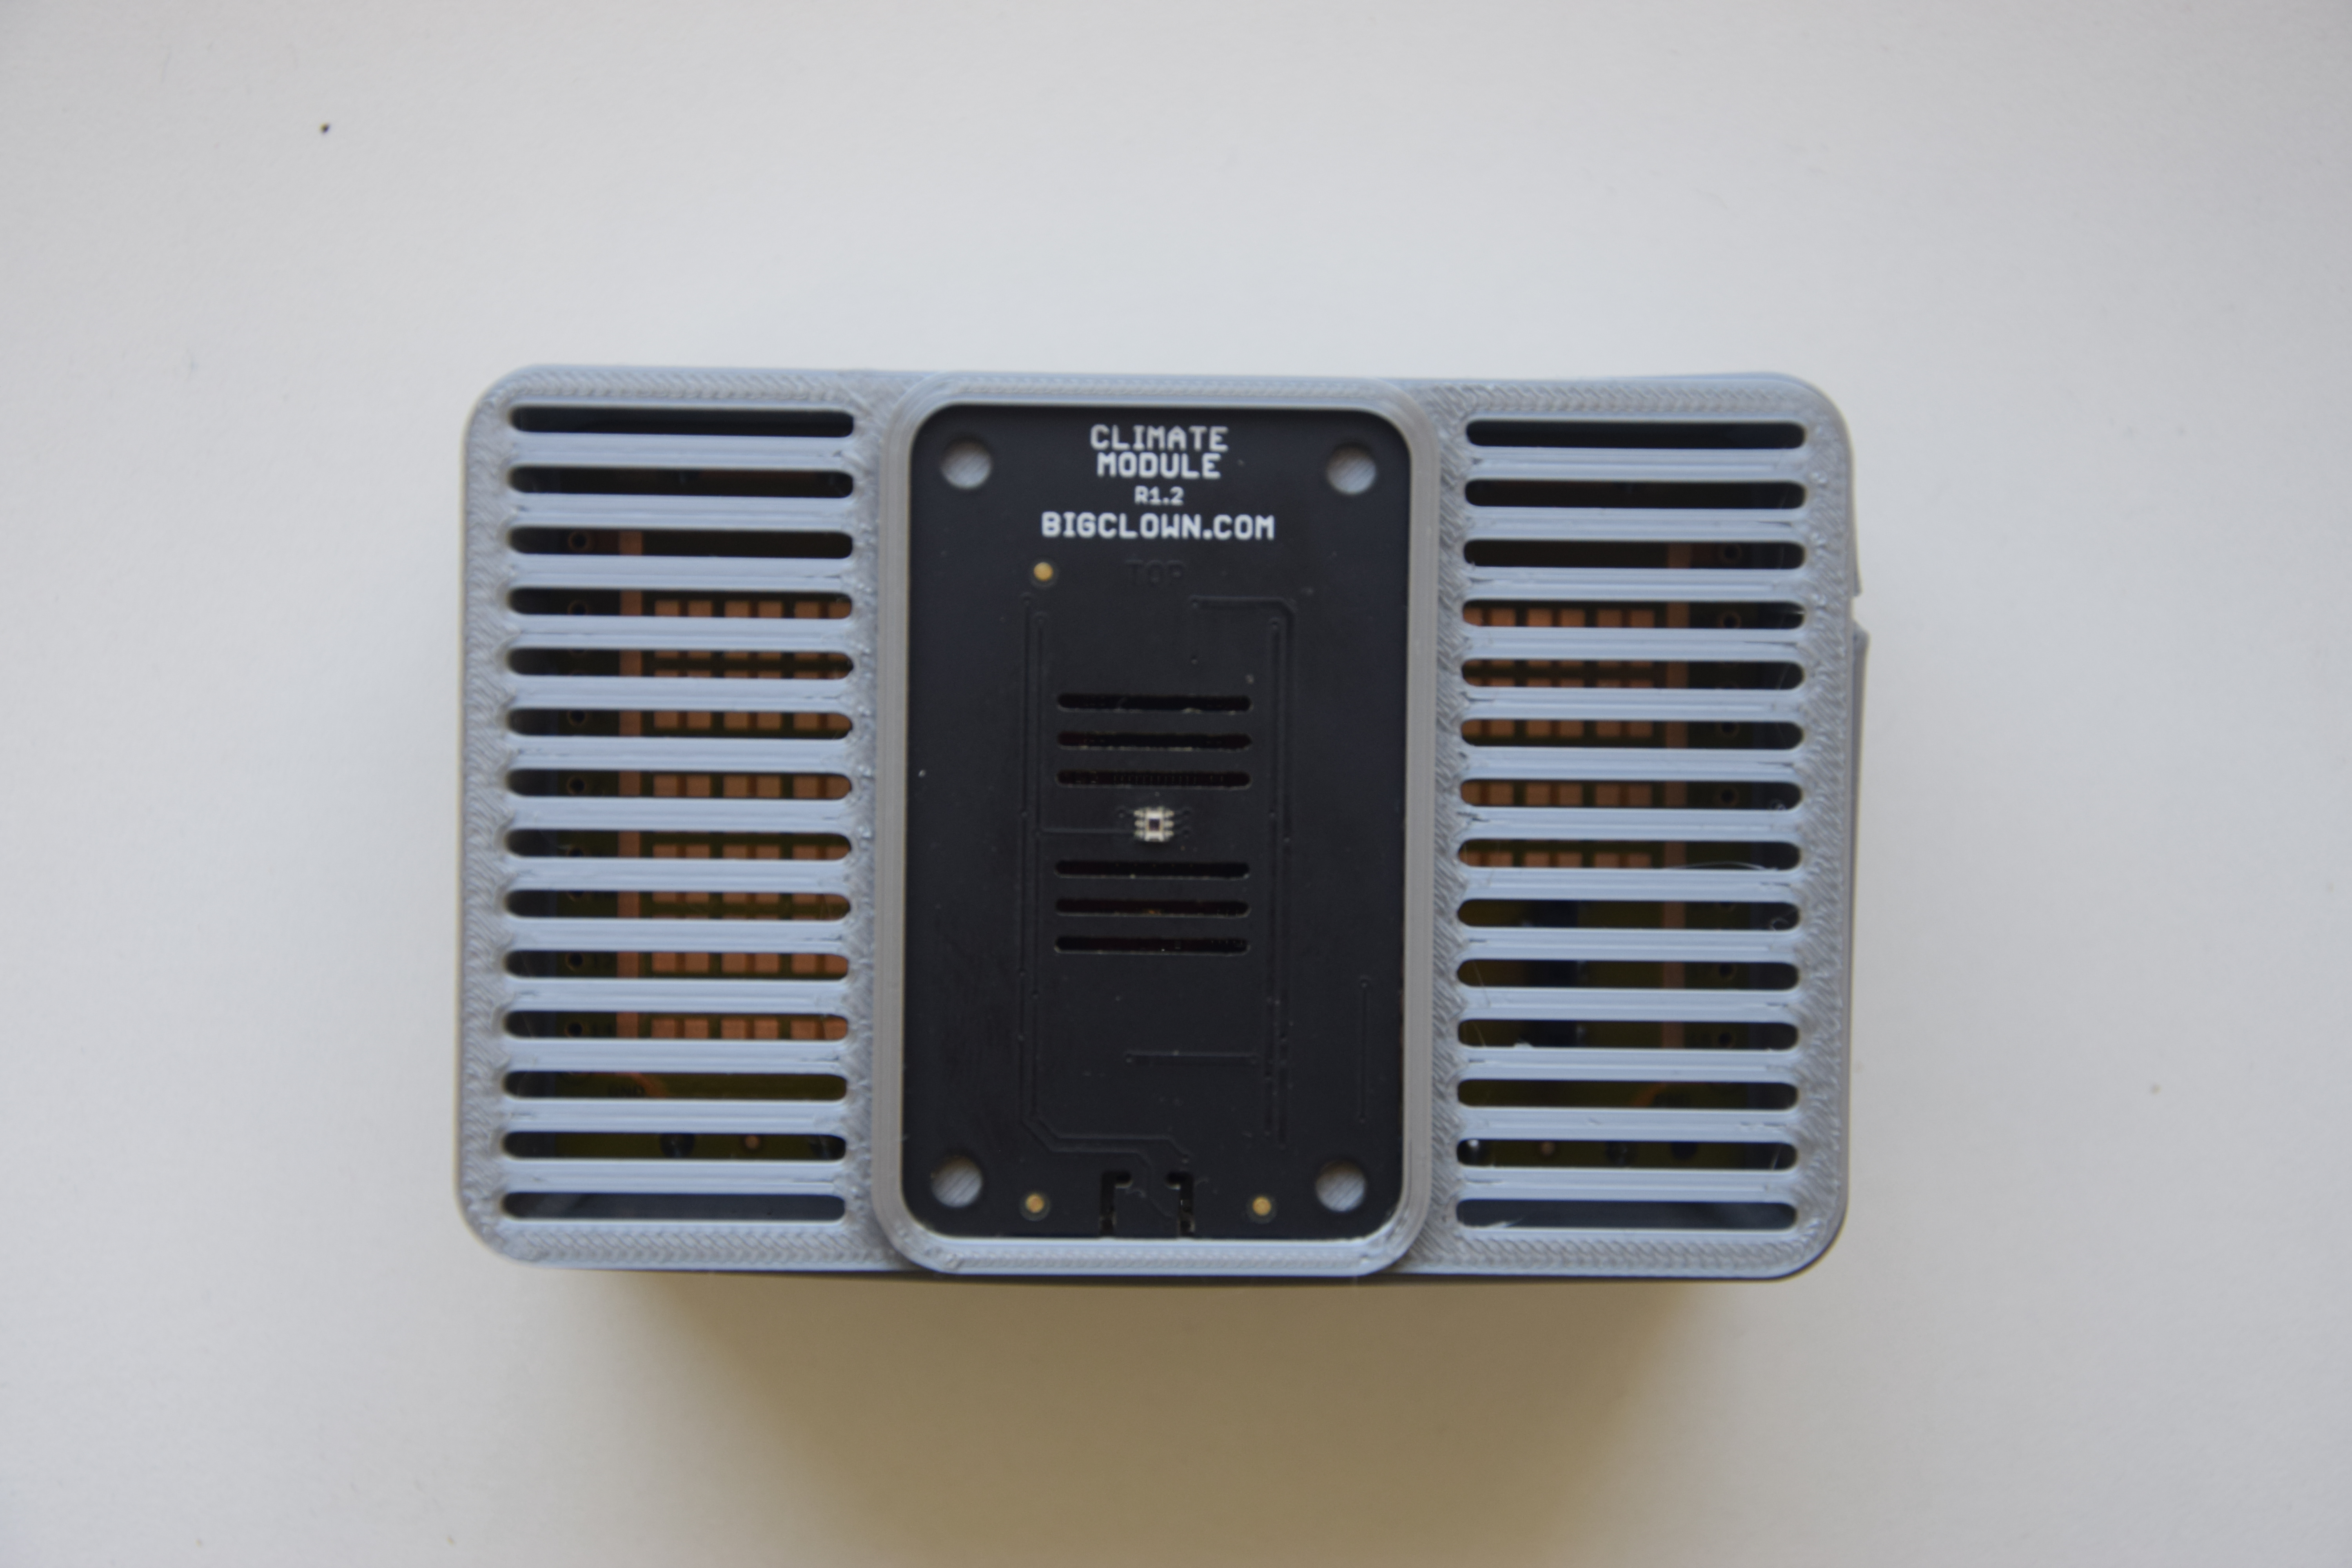
\includegraphics[width=\textwidth]{obrazky-figures/hardwarePhotos/climateMonitor.JPG}
    \caption{Monitor klimatických podmínek pro indoor či outdoor. Foto autor}
    \label{completeClimateMonitor}
  \end{minipage}
  \hfill
  \begin{minipage}[b]{0.4\textwidth}
    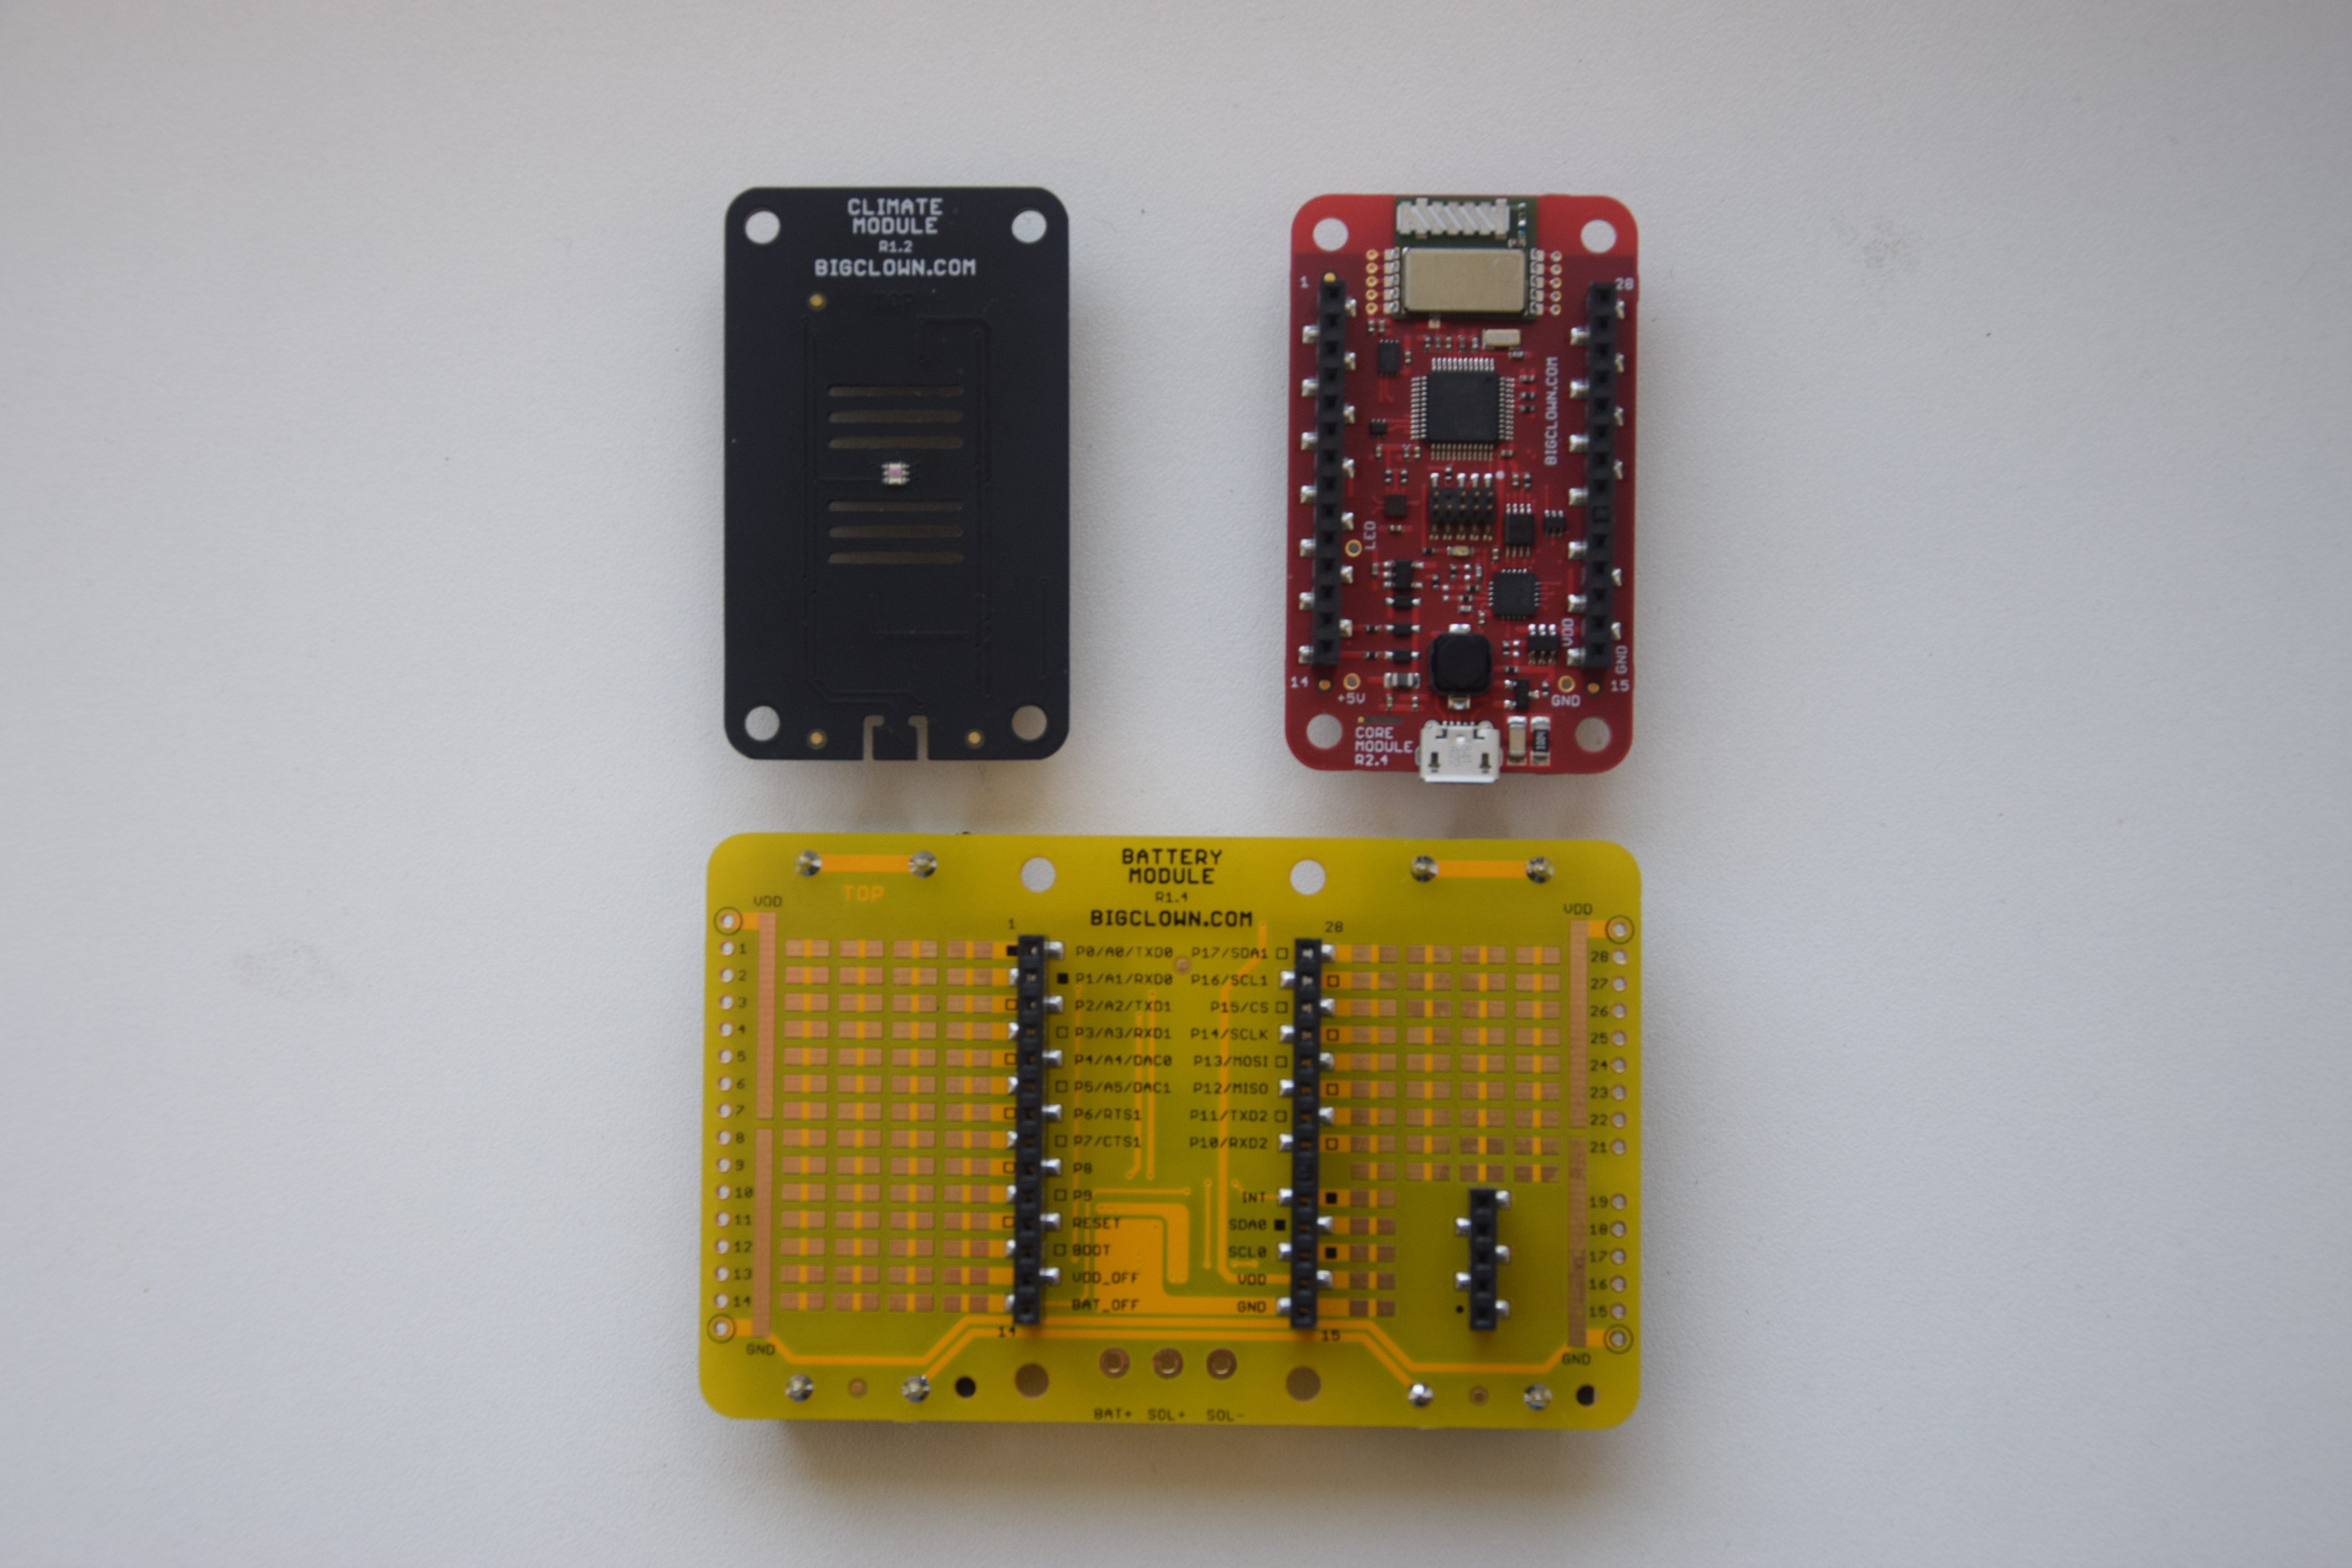
\includegraphics[width=\textwidth]{obrazky-figures/hardwarePhotos/climateMonitorParts.JPG}
    \caption{Stejné zařízení rozložené na jednotlivé moduly. Foto autor}
    \label{disasembeledClimateMonitor}
  \end{minipage}
\end{figure}

Na obrázku \ref{disasembeledClimateMonitor} je vidět rozložené zařízení. Žlutý modul je napájecí bateriový modul, červený obsahuje samotný mikroprocesor a ovládá celé zařízení a černý modul se stará o~měření klimatických podmínek. Toto zařízení je složeno a umístěno do vytisknuté krabičky na Obrázku \ref{completeClimateMonitor}.

\begin{figure}[H]
  \begin{minipage}[b]{0.4\textwidth}
    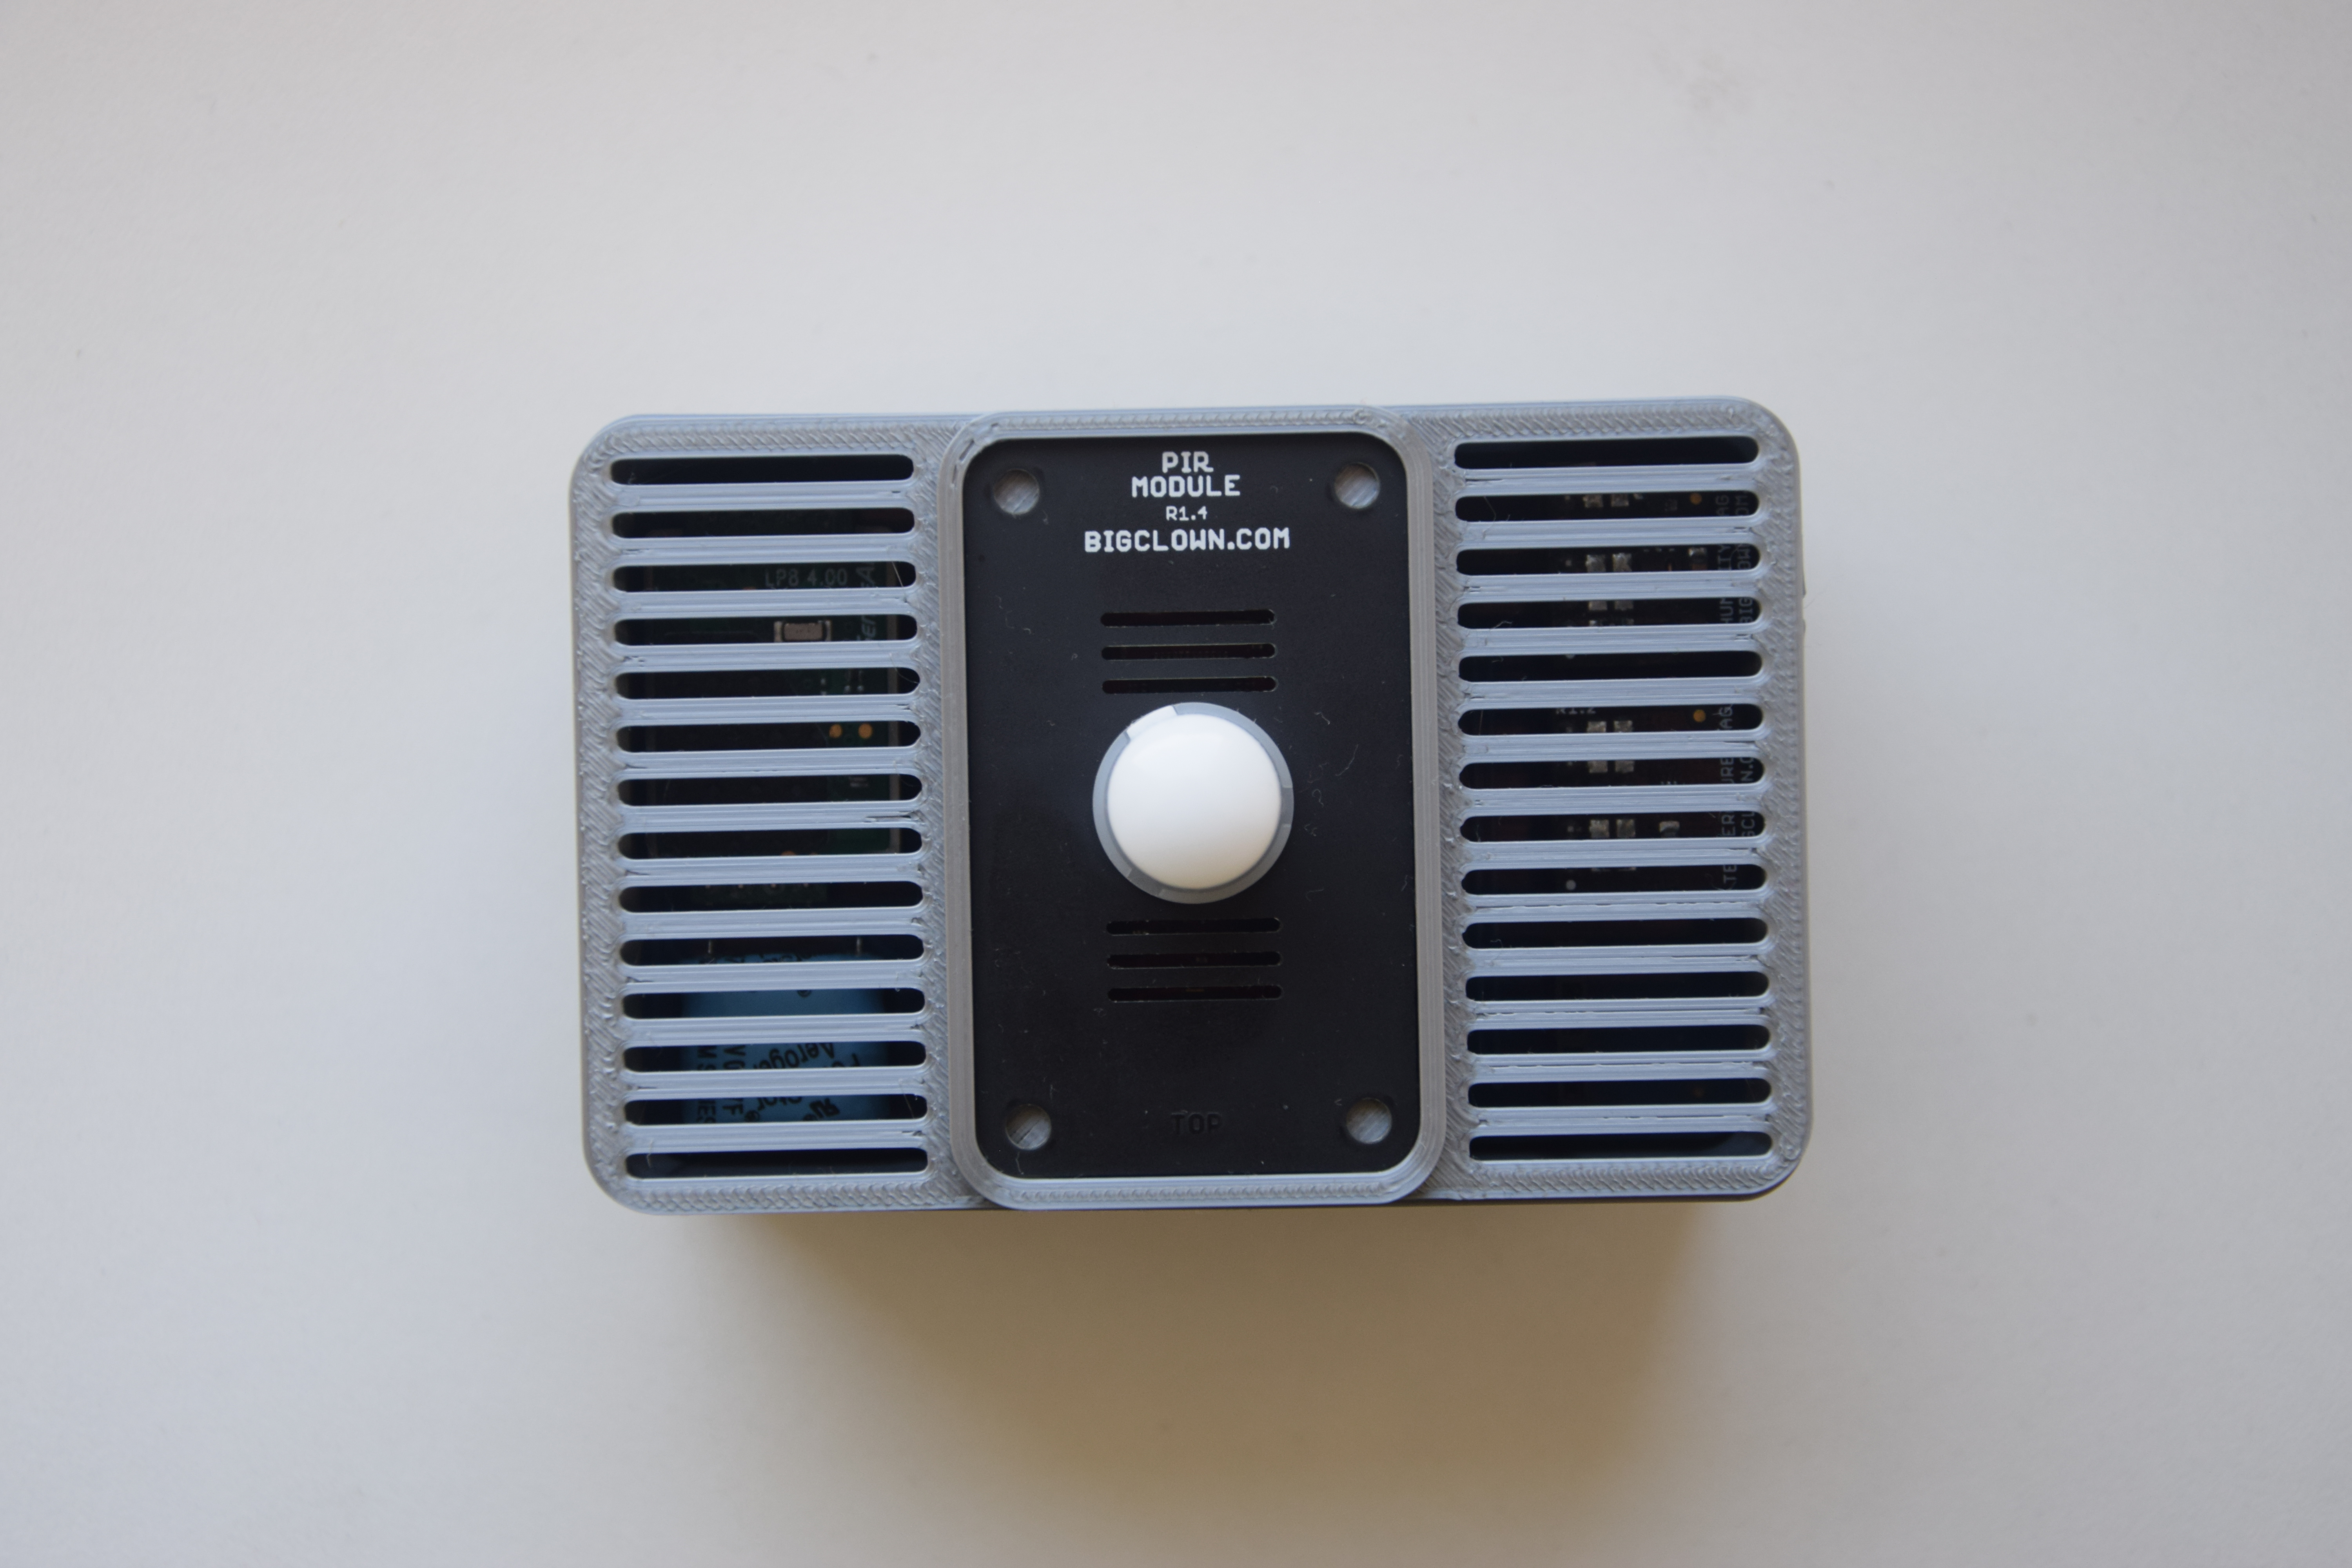
\includegraphics[width=\textwidth]{obrazky-figures/hardwarePhotos/environmentalMonitorWithPIRComplete.JPG}
    \caption{Monitor klimatických podmínek pro indoor s~detektorem pohybu. Foto autor}
    \label{completeCO2Monitor}
  \end{minipage}
  \hfill
  \begin{minipage}[b]{0.4\textwidth}
    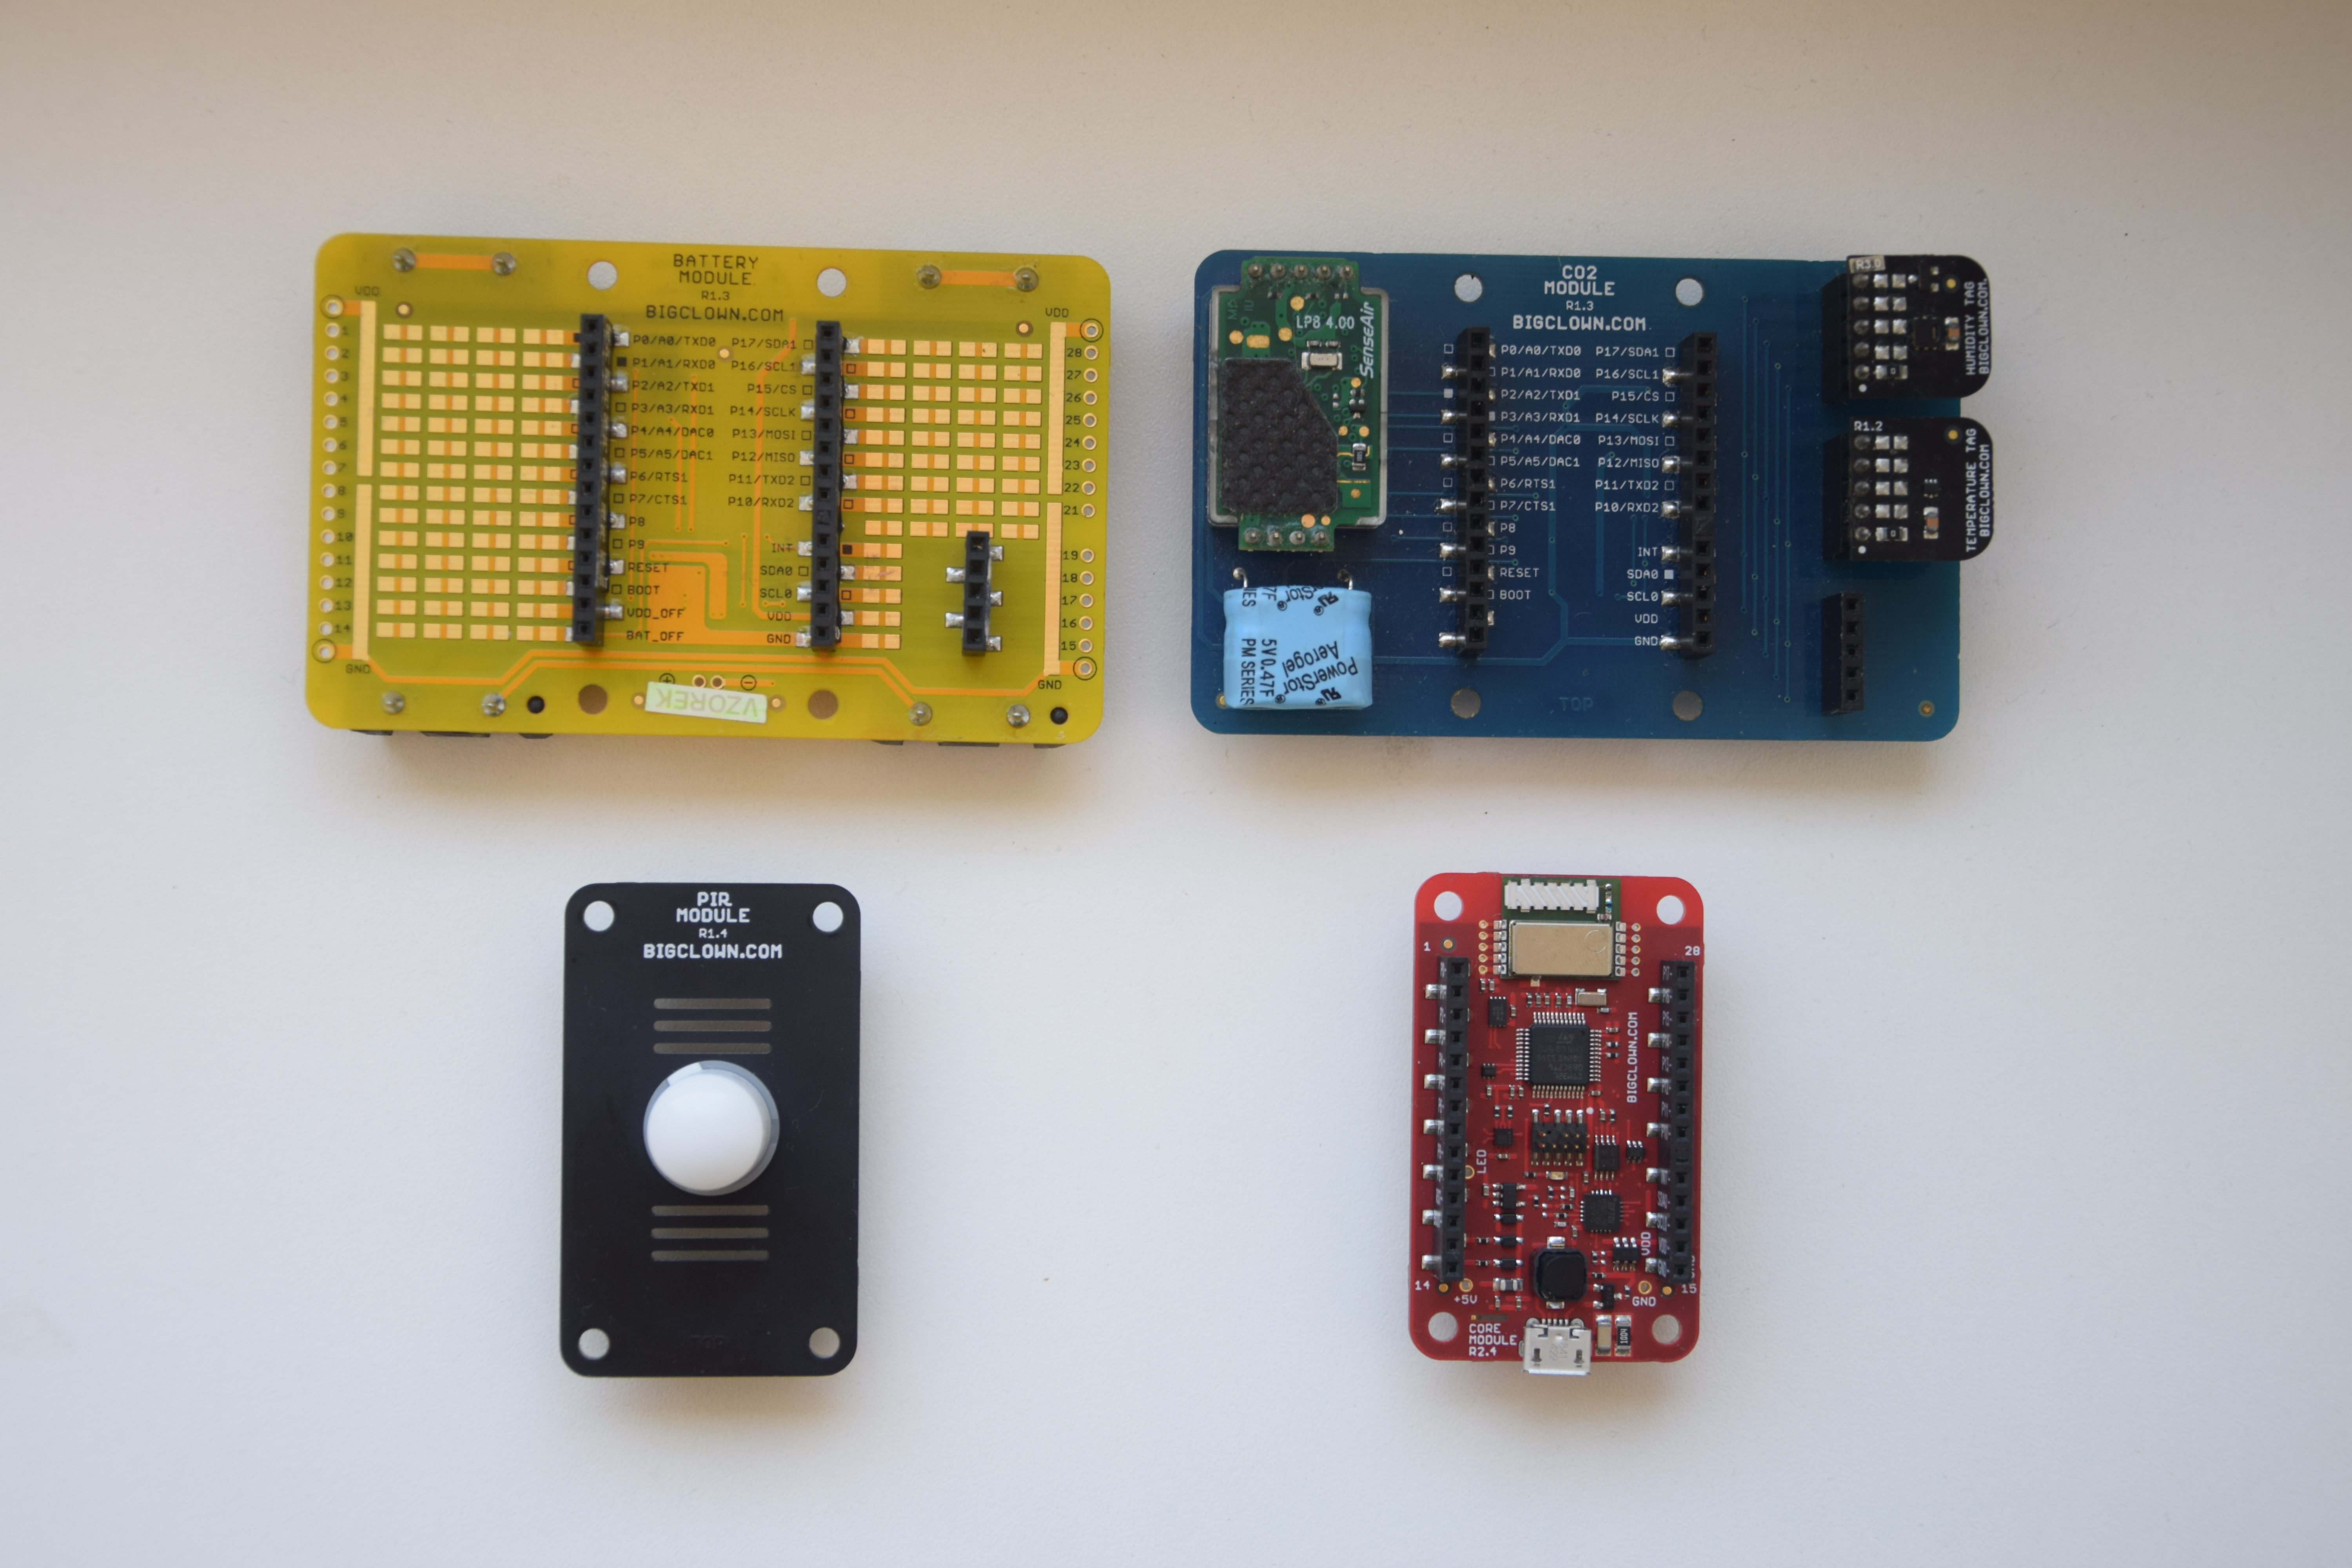
\includegraphics[width=\textwidth]{obrazky-figures/hardwarePhotos/environmentalMonitorWithPIRParts.JPG}
    \caption{Stejné zařízení rozložené na jednotlivé moduly. Foto autor}
    \label{disasembeledCO2Monitor}
  \end{minipage}
\end{figure}

Na obrázku \ref{disasembeledCO2Monitor} je vidět rozložené zařízení. Žlutý modul je napájecí bateriový modul, červený obsahuje samotný mikroprocesor a ovládá celé zařízení a černý modul se stará o~detekci pohybu pomocí PIR čidla. Modrý modul obsahuje měřič $CO_2$ a několik takzvaných tagů pro měření dalších klimatických podmínek. Složené zařízení ve vytisknuté krabičce je možné vidět na Obrázku \ref{completeCO2Monitor}.

\begin{figure}[H]
  \centering
  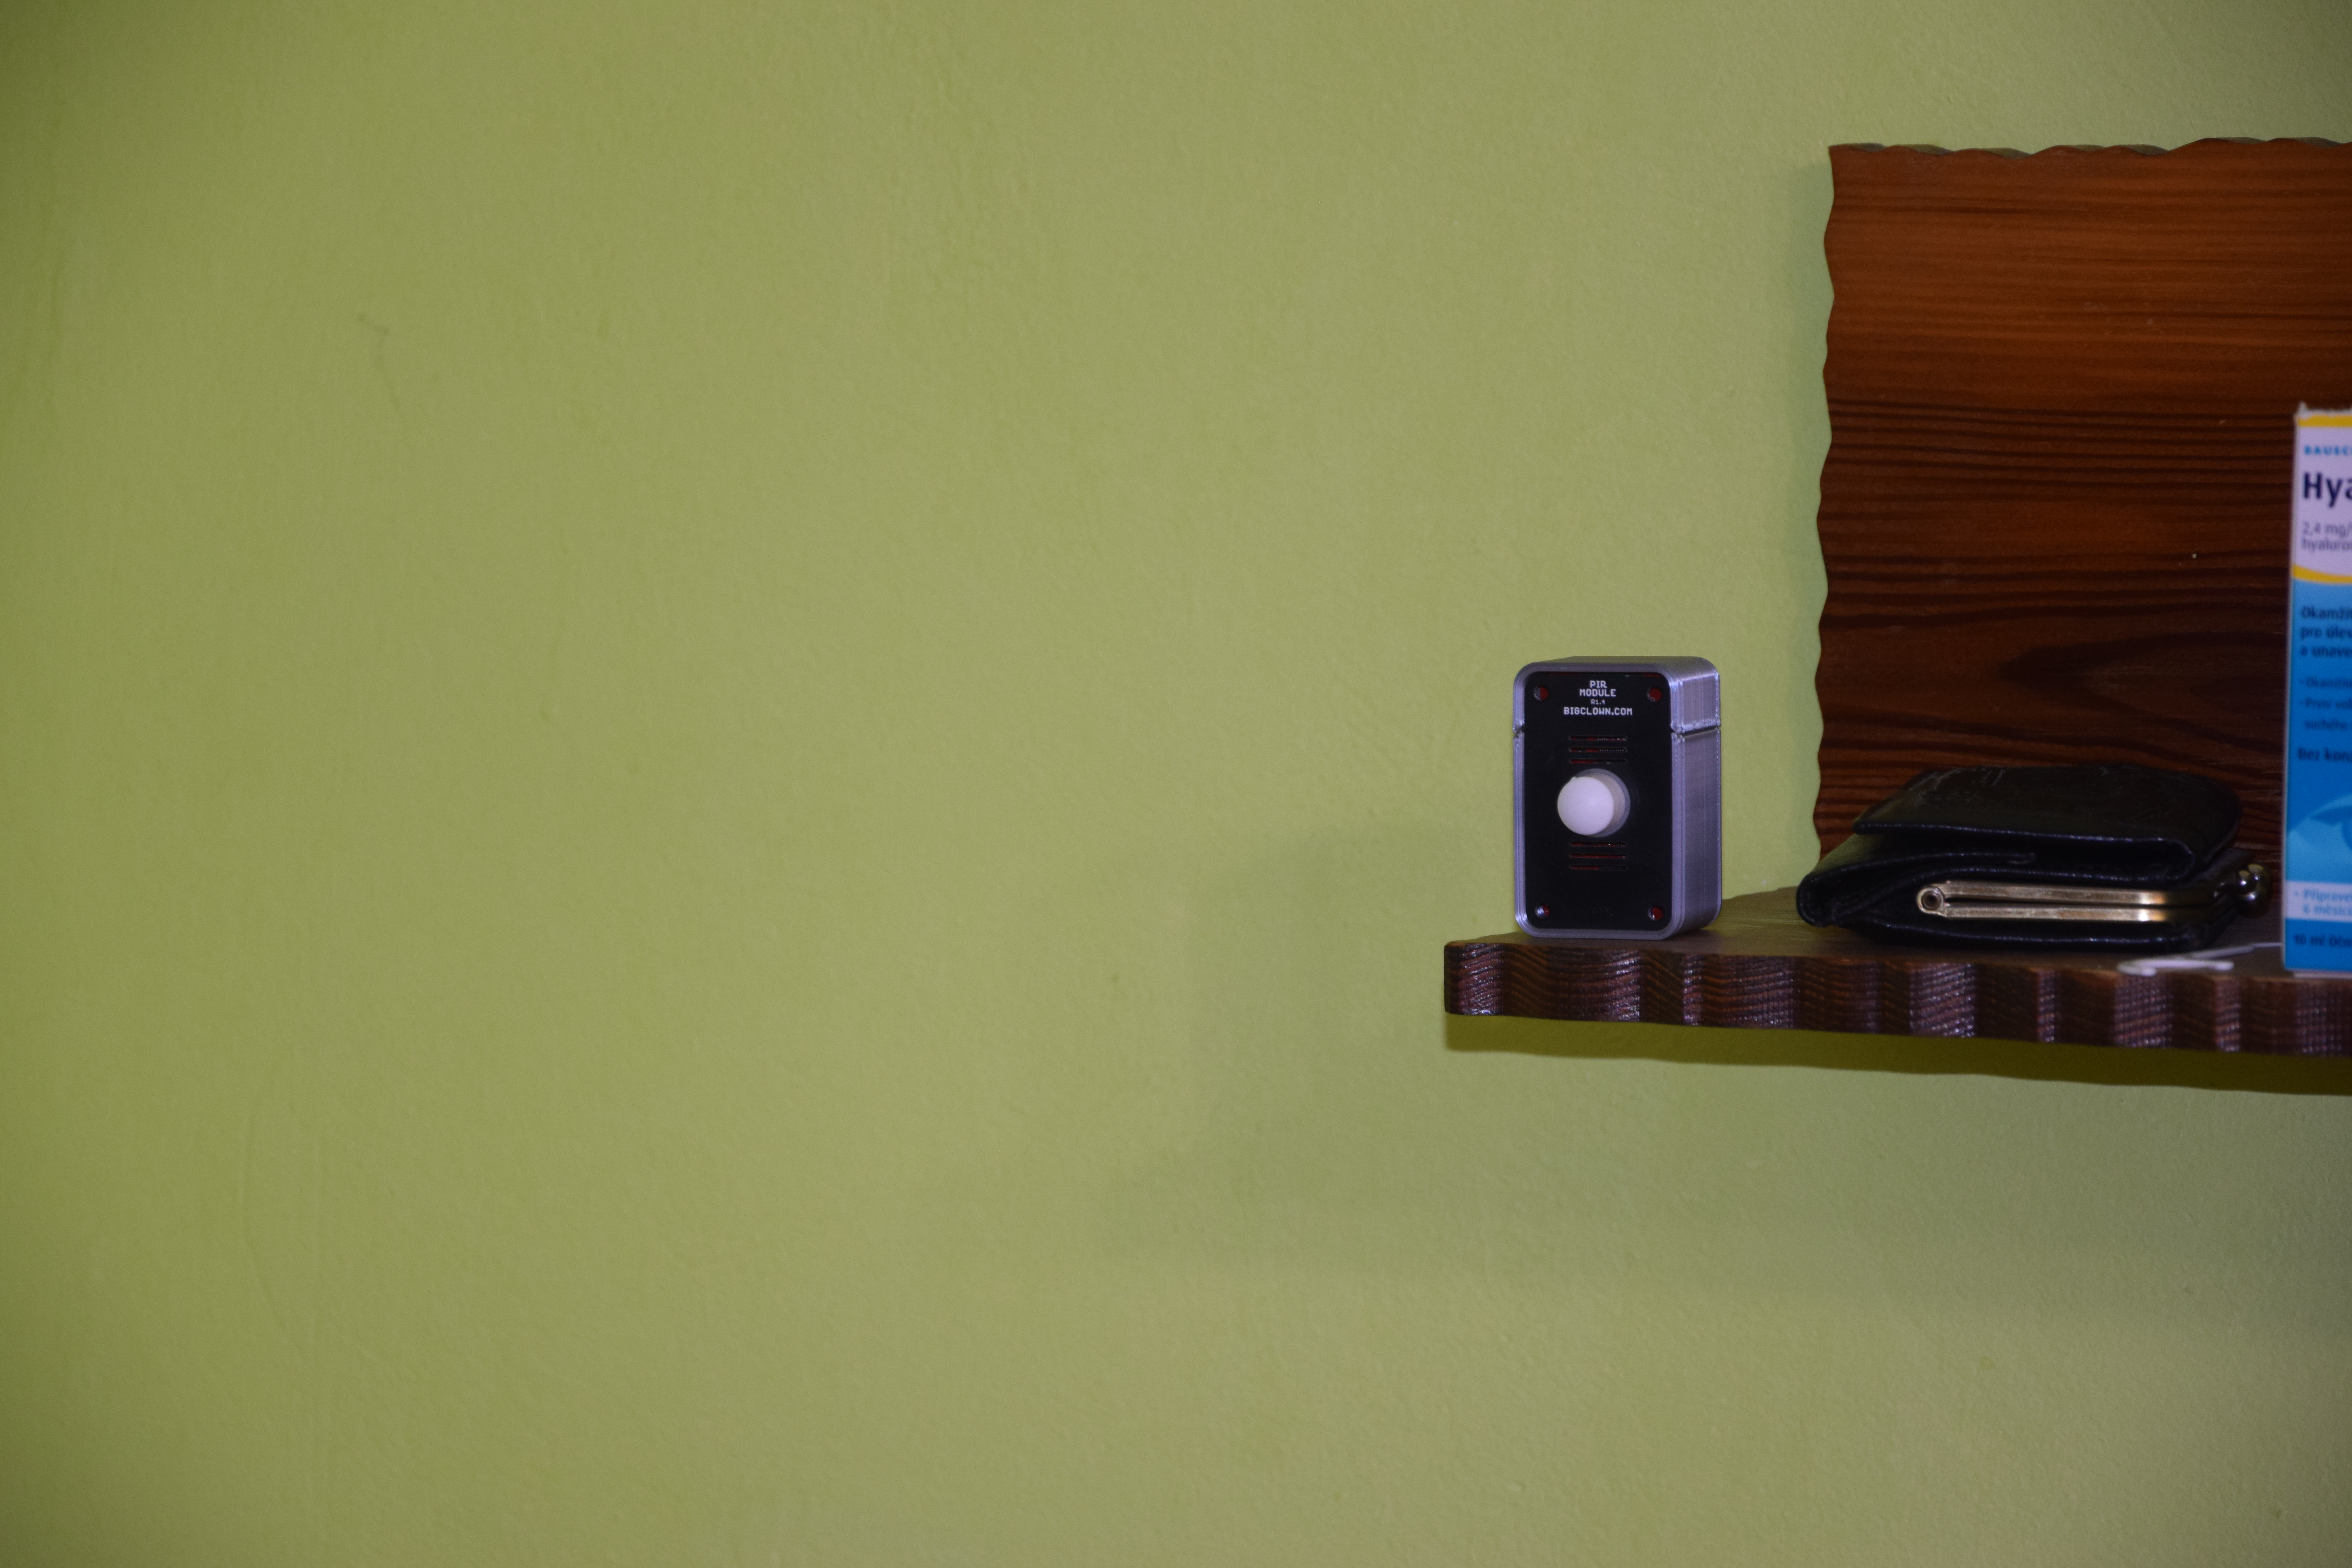
\includegraphics[width=\textwidth]{obrazky-figures/hardwarePhotos/placementShowcase.JPG}
  \caption{Ukázka umístění hardwarového zařízení v~domě. Foto autor}
  \label{placementShowcase}
\end{figure}

Na Obrázku \ref{placementShowcase} je možné vidět ukázku umístění jednoho z~vytvořených hardwarových zařízení. DAlší zařízení jako monitor CO2 či klimatických podmínek mohou být umístěna podobně. Zařízení s~PIR čidlem by měla být umístěna tak aby pokrývyla většinu místnosti.
  \fi
  
  % Kompilace po částech (viz výše, nutno odkomentovat)
  % Compilation piecewise (see above, it is necessary to uncomment it)
  %\subfile{xsmejk28-navrh-a-realizace-IoT-pro-chytrou-domacnost-30-prilohy-appendices}
  
\end{document}
